\documentclass[a4paper]{article}

% CJK support: prefer ctex, fallback to XeTeX native line breaking
\IfFileExists{ctex.sty}{
  \usepackage[fontset=fandol]{ctex}
}{
  % Fallback for minimal TeX installs (e.g. MacTeX Basic, TeX Live scheme-basic)
  % without ctex/xeCJK. Uses XeTeX's built-in CJK line breaking.
  \usepackage{fontspec}
  \XeTeXlinebreaklocale "zh"
  \XeTeXlinebreakskip = 0pt plus 1pt
  \IfFontExistsTF{Songti SC}{\setmainfont{Songti SC}}{%
    \IfFontExistsTF{Noto Serif CJK SC}{\setmainfont{Noto Serif CJK SC}}{}%
  }
  \IfFontExistsTF{Heiti SC}{\setsansfont{Heiti SC}}{%
    \IfFontExistsTF{Noto Sans CJK SC}{\setsansfont{Noto Sans CJK SC}}{}%
  }
}

% Basic packages
\usepackage{amsmath, amssymb}
\usepackage{graphicx}
\usepackage[margin=2.5cm]{geometry}
\emergencystretch=3em
\usepackage[most]{tcolorbox}
\usepackage{etoolbox}
\usepackage{listings}
\usepackage{hyperref}
\usepackage{booktabs}
\usepackage{array}
\usepackage{subcaption}
\usepackage{float}
\usepackage{tikz}
\IfFileExists{pgfplots.sty}{
    \usepackage{pgfplots}
    \pgfplotsset{compat=1.18}
}{}

% ===== Highlight boxes =====
\newtcolorbox{knowledgebox}[1]{
    enhanced, colback=blue!5!white, colframe=blue!75!black, colbacktitle=blue!75!black,
    coltitle=white, fonttitle=\bfseries, title={#1}, attach boxed title to top left={yshift=-2mm, xshift=2mm},
    boxrule=1pt, sharp corners
}

\newtcolorbox{importantbox}[1]{
    enhanced, colback=yellow!10!white, colframe=yellow!80!black, colbacktitle=yellow!80!black,
    coltitle=black, fonttitle=\bfseries, title={#1}, sharp corners
}

\newtcolorbox{warningbox}[1]{
    enhanced, colback=red!5!white, colframe=red!75!black, colbacktitle=red!75!black,
    coltitle=white, fonttitle=\bfseries, title={#1}, sharp corners
}

\newtcolorbox{practicebox}[1]{
    enhanced, colback=black!3!white, colframe=black!75, colbacktitle=black!75,
    coltitle=white, fonttitle=\bfseries, title={#1}, sharp corners
}

% ===== Code listings =====
\lstset{
    basicstyle=\ttfamily\small,
    keywordstyle=\color{blue},
    stringstyle=\color{red!60!black},
    commentstyle=\color{green!60!black},
    breaklines=true,
    frame=single,
    numbers=left,
    numberstyle=\tiny\color{gray},
    captionpos=b,
    extendedchars=false
}

% ===== Figure provenance and unit macros =====
% \vtag goes inside \caption{...}; \srcnote{MM:SS--MM:SS} follows the figure environment.
\newcommand{\vtag}{\protect\footnotemark}
\newcommand{\srcnote}[1]{\footnotetext{视频画面时间区间：#1。若为裁剪图，时间区间仍对应原视频画面。}}
% Units work in text and math mode; never hand-write $^\circ$ or \AA inside \mathrm.
\newcommand{\degC}{\ensuremath{^{\circ}\mathrm{C}}}
\newcommand{\um}{\ensuremath{\mu\mathrm{m}}}
\newcommand{\nm}{\ensuremath{\mathrm{nm}}}
\newcommand{\angstrom}{\ensuremath{\text{\AA}}}

% ===== Front-page metadata =====
% Fill these in when generating notes.
\newcommand{\notetitle}{微分方程}
\newcommand{\notesubtitle}{GAMES001 图形学中的数学 · 第 12 集：常微分方程、偏微分方程、球谐函数与格林函数}
\newcommand{\noteauthors}{根据 GAMES-Webinar 直播录像整理（倪星宇 主讲）}
\newcommand{\notedate}{2024年6月3日（直播）}
\newcommand{\videochannel}{GAMES-Webinar（哔哩哔哩）}
\newcommand{\videopublishdate}{2024年3月6日（合集）}
\newcommand{\videoduration}{1小时6分7秒}
\newcommand{\videourl}{https://www.bilibili.com/video/BV1MF4m1V7e3/?p=12}
\newcommand{\videocoverpath}{cover.jpg}

\begin{document}

% ===== Title page =====
\begin{titlepage}
\centering
{\Large 课程笔记\par}
\vspace{1.2cm}
{\huge\bfseries \notetitle\par}
\ifdefempty{\notesubtitle}{}{
\vspace{0.3cm}
{\large \notesubtitle\par}
}
\vspace{0.5cm}
{\large \noteauthors\par}
\vspace{0.3cm}
{\large \notedate\par}
\vspace{1.0cm}

\ifdefempty{\videocoverpath}{
{\small 请在生成笔记时填入视频封面图的本地路径。\par}
}{
\includegraphics[width=0.82\textwidth,height=0.40\textheight,keepaspectratio]{\videocoverpath}\par
}

\vfill
\begin{tcolorbox}[width=0.9\textwidth, colback=black!2!white, colframe=black!60, sharp corners]
\textbf{视频作者/频道}：\videochannel\par
\textbf{发布日期}：\videopublishdate\par
\textbf{视频时长}：\videoduration\par
\textbf{视频链接}：
\ifdefempty{\videourl}{
未填写
}{
\href{\videourl}{\nolinkurl{\videourl}}
}
\end{tcolorbox}
\end{titlepage}

\tableofcontents
\newpage

%% --- 正文内容开始 --- %%

\section{这一讲讲什么}

第十二讲由倪星宇主讲，主题是微分方程（differential equations）。讲者说，按照课程大纲，前面讲了场论、概率等内容，今天的微分方程是连续数学部分的最后一节课；下一讲开始进入离散的部分，会讲线性求解器。所以这节课要起到承上启下的作用。

图形学中的微分方程相当多，从常微分方程到偏微分方程，各种各样的方程都需要求解。讲者坦言，一节课不可能把图形学涉及的微分方程知识都讲到，只能挂一漏万，挑最重要的方法来讲。

本讲的路线是：先介绍微分方程的基本概念；再讲常微分方程的几类解法（可分离变量、一阶线性、伯努利方程、可降阶的高阶方程、二阶常系数线性方程）；然后讲二阶偏微分方程的分类和三个典型方程；接着介绍分离变量法，并用它在球坐标下解拉普拉斯方程得到球谐函数；再介绍格林函数法；最后讲微分方程的数值解。

\begin{importantbox}{本讲的主线}
讲者概括了四类求解方法：通解法，根据特定微分方程的通解代值求特解；分离变量法，数学家、物理学家也常用；格林函数法，是从数学到计算机的桥梁，因为计算机里很多时候求的就是格林函数；数值法，它本身就是计算机图形学研究的核心之一，如果你发明了一种更好的数值方法去求解某类微分方程，那就是图形学的重要贡献。
\end{importantbox}

\section{微分方程的基本概念}

\noindent\begin{minipage}{\textwidth}
\begin{figure}[H]
\centering
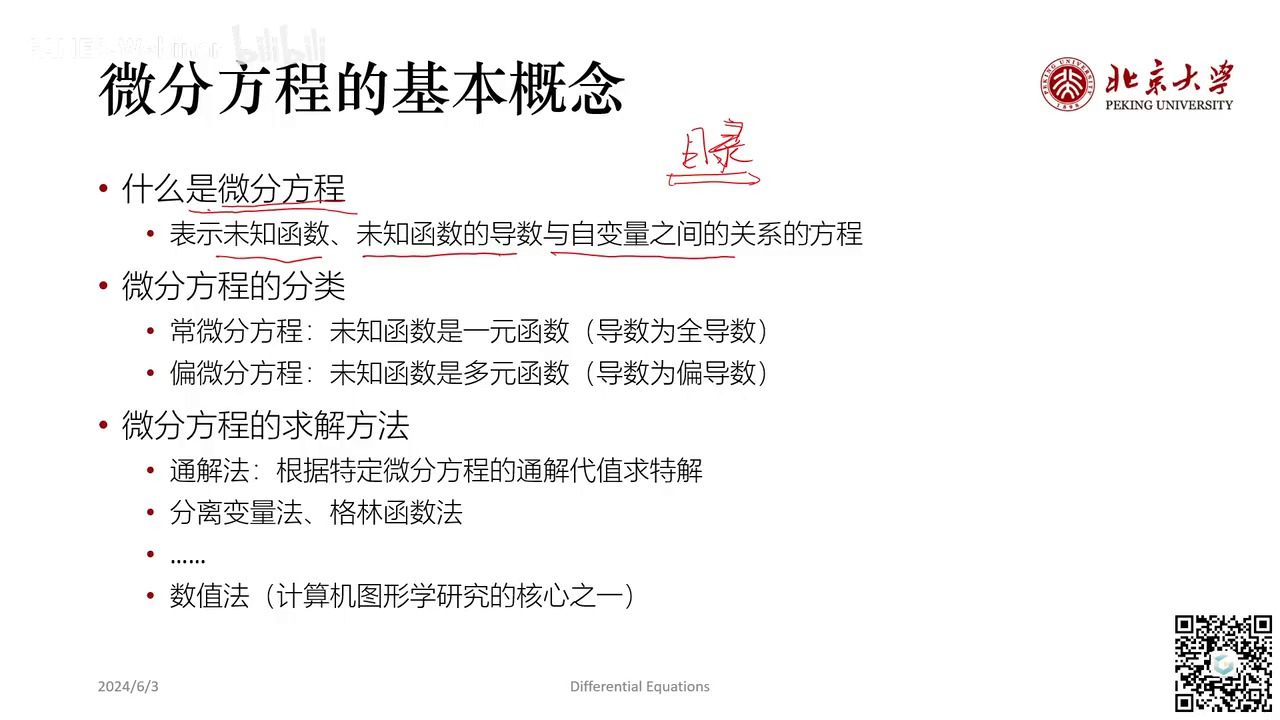
\includegraphics[width=0.92\textwidth]{figures/fig_01_basics.jpg}
\caption{微分方程的基本概念：定义、分类与求解方法\vtag}
\end{figure}
\srcnote{00:03:15--00:03:30}
\end{minipage}


微分方程是表示未知函数、未知函数的导数与自变量之间的关系的方程，这里的导数可以是一阶、二阶等各阶导数。按未知函数的类型分为两类：常微分方程，未知函数是一元函数，导数为全导数；偏微分方程，未知函数是多元函数，导数为偏导数，用偏导符号 $\partial$ 表示。

讲者提到，对于修过数学分析的同学来说，常微分方程部分应该比较熟悉；对大一同学来说，可能刚学到。

\section{常微分方程}

\subsection{可分离变量的微分方程}

\noindent\begin{minipage}{\textwidth}
\begin{figure}[H]
\centering
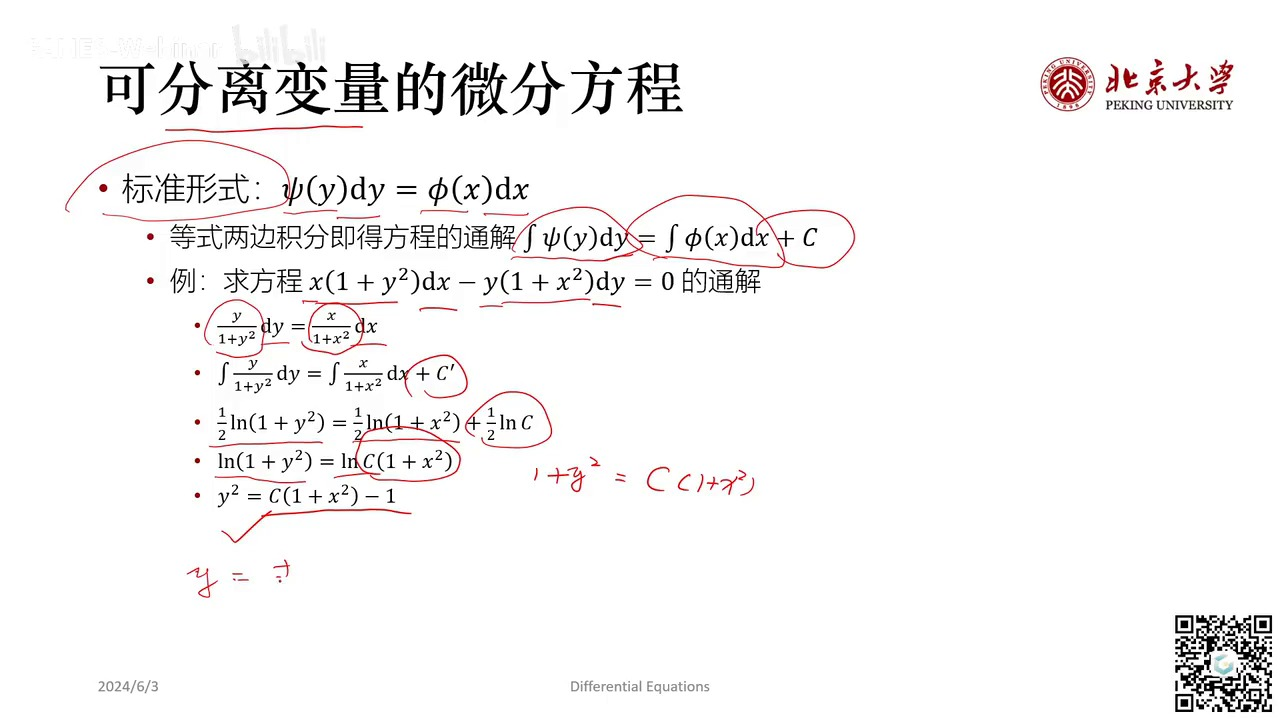
\includegraphics[width=0.92\textwidth]{figures/fig_02_separable.jpg}
\caption{可分离变量的微分方程及例题\vtag}
\end{figure}
\srcnote{00:08:00--00:08:15}
\end{minipage}


标准形式为 $\psi(y)\,\mathrm{d}y=\phi(x)\,\mathrm{d}x$。等式两边积分，即得方程的通解
\begin{equation}
\int\psi(y)\,\mathrm{d}y=\int\phi(x)\,\mathrm{d}x+C .
\end{equation}

例：求方程 $x(1+y^2)\,\mathrm{d}x-y(1+x^2)\,\mathrm{d}y=0$ 的通解。分离变量得 $\frac{y}{1+y^2}\mathrm{d}y=\frac{x}{1+x^2}\mathrm{d}x$，两边积分：
\begin{equation}
\frac{1}{2}\ln(1+y^2)=\frac{1}{2}\ln(1+x^2)+\frac{1}{2}\ln C .
\end{equation}
讲者解释，积分后还差一个常数，为了化简方便把它写成 $\frac{1}{2}\ln C$。于是 $\ln(1+y^2)=\ln C(1+x^2)$，即 $y^2=C(1+x^2)-1$。如果想写成 $y$ 是 $x$ 的函数的形式，也可以写成 $y=\pm\sqrt{C(1+x^2)-1}$。

\subsection{一阶线性微分方程}

\noindent\begin{minipage}{\textwidth}
\begin{figure}[H]
\centering
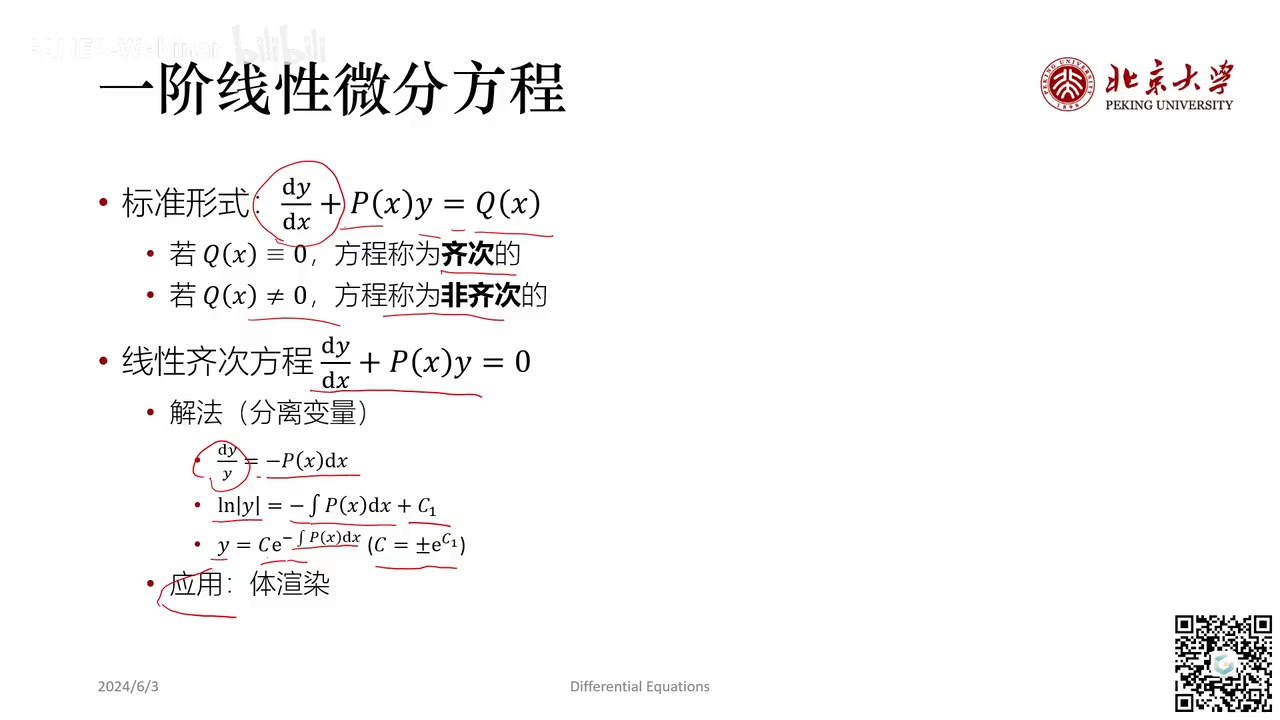
\includegraphics[width=0.92\textwidth]{figures/fig_03_linear1.jpg}
\caption{一阶线性微分方程：齐次方程的分离变量解法\vtag}
\end{figure}
\srcnote{00:09:45--00:10:00}
\end{minipage}


标准形式为
\begin{equation}
\frac{\mathrm{d}y}{\mathrm{d}x}+P(x)y=Q(x).
\end{equation}
若 $Q(x)\equiv 0$，方程称为齐次的；若 $Q(x)\not\equiv 0$，方程称为非齐次的。

线性齐次方程 $\frac{\mathrm{d}y}{\mathrm{d}x}+P(x)y=0$ 很容易分离变量：两边先乘以 $\mathrm{d}x$ 再除以 $y$，得 $\frac{\mathrm{d}y}{y}=-P(x)\mathrm{d}x$；两端积分得 $\ln|y|=-\int P(x)\mathrm{d}x+C_1$；再取指数，
\begin{equation}
y=Ce^{-\int P(x)\,\mathrm{d}x},\qquad C=\pm e^{C_1}.
\end{equation}
课件上标注的应用是体渲染。

\begin{knowledgebox}{一阶线性方程与体渲染}
讲义作者补充：光在参与介质中传播时，辐亮度 $L$ 沿光线方向的变化满足 $\frac{\mathrm{d}L}{\mathrm{d}s}=-\sigma_t(s)L$，正是上面的齐次方程，解为 $L(s)=L(0)e^{-\int_0^s\sigma_t\,\mathrm{d}s'}$，即比尔—朗伯定律，指数中的积分称为光学厚度。若再考虑介质自发光或内散射，方程右端多出一个源项，就成了非齐次方程，其解正是下面常数变易法给出的形式。
\end{knowledgebox}

线性非齐次方程与齐次方程的唯一区别是右端有函数 $Q(x)$，不再是零。用待定系数法（常数变易法）求解：把齐次解中的常数 $C$ 换成函数 $C(x)$，令 $y=C(x)e^{-\int P(x)\mathrm{d}x}$，则
\begin{equation}
y'=C'(x)e^{-\int P(x)\mathrm{d}x}+C(x)e^{-\int P(x)\mathrm{d}x}\big[-P(x)\big].
\end{equation}
代入原方程，含 $C(x)$ 的项恰好与 $P(x)y$ 抵消，得到 $C'(x)e^{-\int P(x)\mathrm{d}x}=Q(x)$，即 $C(x)=\int Q(x)e^{\int P(x)\mathrm{d}x}\mathrm{d}x+C$。于是
\begin{equation}
y=e^{-\int P(x)\,\mathrm{d}x}\left[\int Q(x)e^{\int P(x)\,\mathrm{d}x}\mathrm{d}x+C\right].
\end{equation}

\noindent\begin{minipage}{\textwidth}
\begin{figure}[H]
\centering
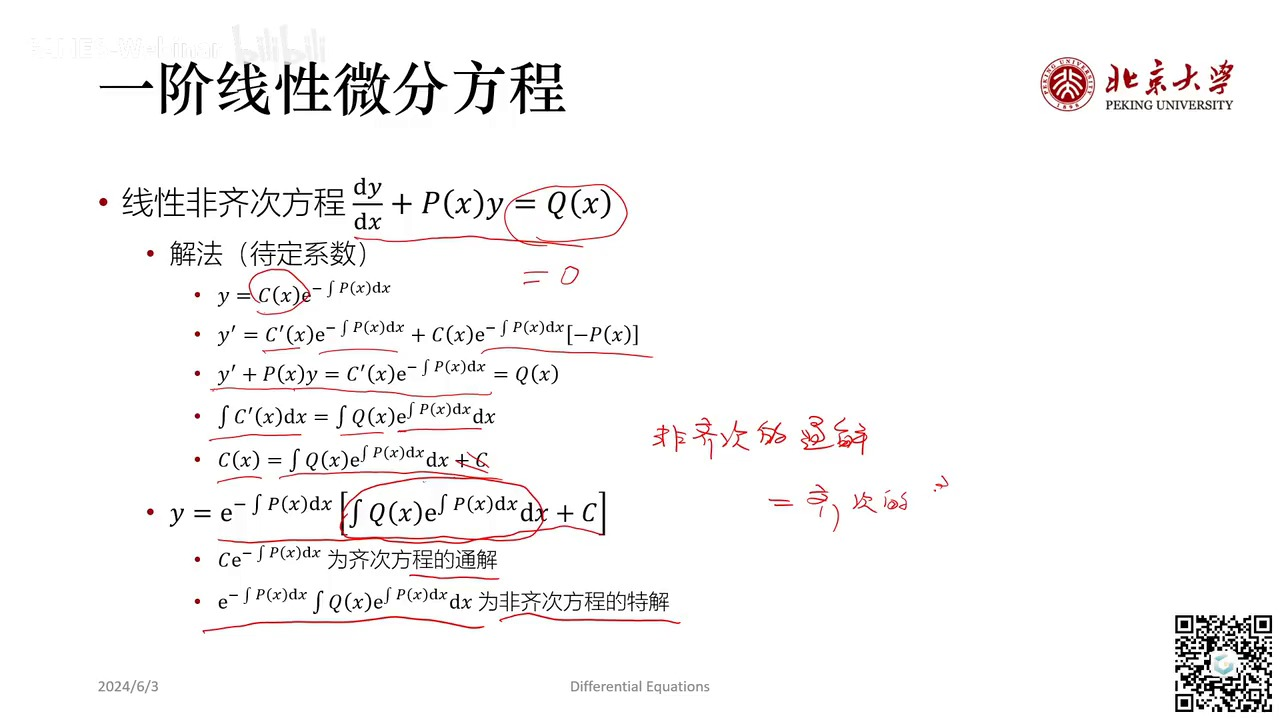
\includegraphics[width=0.92\textwidth]{figures/fig_04_linear1_note.jpg}
\caption{讲者在非齐次方程通解旁标注齐次通解与非齐次特解\vtag}
\end{figure}
\srcnote{00:12:30--00:12:45}
\end{minipage}


展开后，$Ce^{-\int P(x)\mathrm{d}x}$ 是齐次方程的通解，$e^{-\int P(x)\mathrm{d}x}\int Q(x)e^{\int P(x)\mathrm{d}x}\mathrm{d}x$ 是非齐次方程的一个特解。讲者说，中间那个不定积分加不加常数不影响结果，可以去掉，它就是非齐次方程的特解。

\begin{importantbox}{通解 = 齐次通解 + 非齐次特解}
这是线性方程的普遍结构：非齐次方程的任意两个解之差满足齐次方程。所以只要找到非齐次方程的一个特解，再加上齐次方程的全部解，就得到非齐次方程的全部解。后面二阶线性方程也遵循同样的结构。
\end{importantbox}

\subsection{伯努利方程}

\noindent\begin{minipage}{\textwidth}
\begin{figure}[H]
\centering
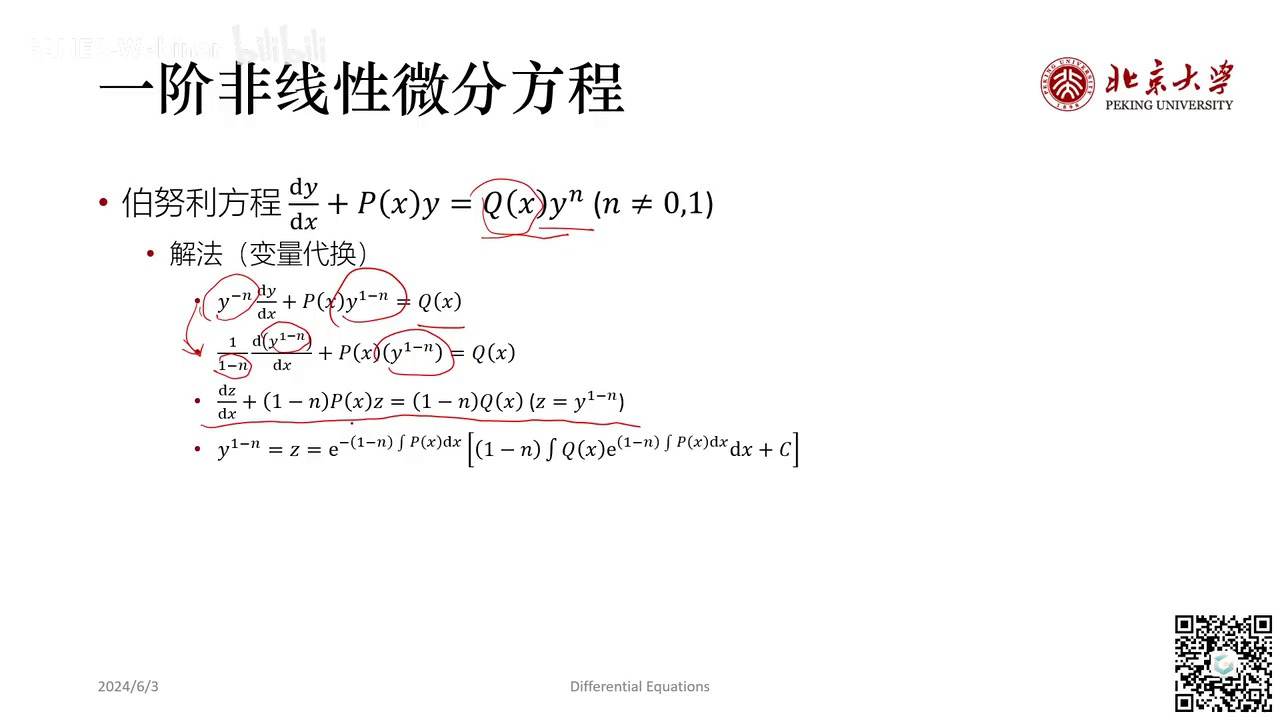
\includegraphics[width=0.92\textwidth]{figures/fig_05_bernoulli.jpg}
\caption{一阶非线性微分方程：伯努利方程与变量代换\vtag}
\end{figure}
\srcnote{00:14:45--00:15:00}
\end{minipage}


下面看一阶非线性微分方程。伯努利方程为
\begin{equation}
\frac{\mathrm{d}y}{\mathrm{d}x}+P(x)y=Q(x)y^n\qquad(n\ne 0,1).
\end{equation}
解法是变量代换。两边同乘 $y^{-n}$：$y^{-n}\frac{\mathrm{d}y}{\mathrm{d}x}+P(x)y^{1-n}=Q(x)$，右边就没有 $y$ 的 $n$ 次幂了。讲者指出，$y^{1-n}$ 对 $x$ 求导恰好得到 $(1-n)y^{-n}\frac{\mathrm{d}y}{\mathrm{d}x}$，只多了一个常数因子。所以
\begin{equation}
\frac{1}{1-n}\frac{\mathrm{d}(y^{1-n})}{\mathrm{d}x}+P(x)y^{1-n}=Q(x).
\end{equation}
令 $z=y^{1-n}$，得 $\frac{\mathrm{d}z}{\mathrm{d}x}+(1-n)P(x)z=(1-n)Q(x)$，这是关于 $z$ 的一阶线性方程，用上一节的公式即得
\begin{equation}
y^{1-n}=z=e^{-(1-n)\int P(x)\mathrm{d}x}\left[(1-n)\int Q(x)e^{(1-n)\int P(x)\mathrm{d}x}\mathrm{d}x+C\right].
\end{equation}
讲者总结，到这里已经展示了求解微分方程的几种方法：分离变量法、待定系数法、变量代换法。

\begin{warningbox}{为什么要求 $n\ne 0,1$}
讲义作者提醒：当 $n=0$ 时，伯努利方程就是一阶线性非齐次方程；当 $n=1$ 时，它变成 $y'+[P(x)-Q(x)]y=0$，是可分离变量的齐次方程。这两种情况已经有更直接的解法，而且代换 $z=y^{1-n}$ 在 $n=1$ 时退化为常数，无法使用。
\end{warningbox}

\subsection{可降阶的高阶微分方程}

\noindent\begin{minipage}{\textwidth}
\begin{figure}[H]
\centering
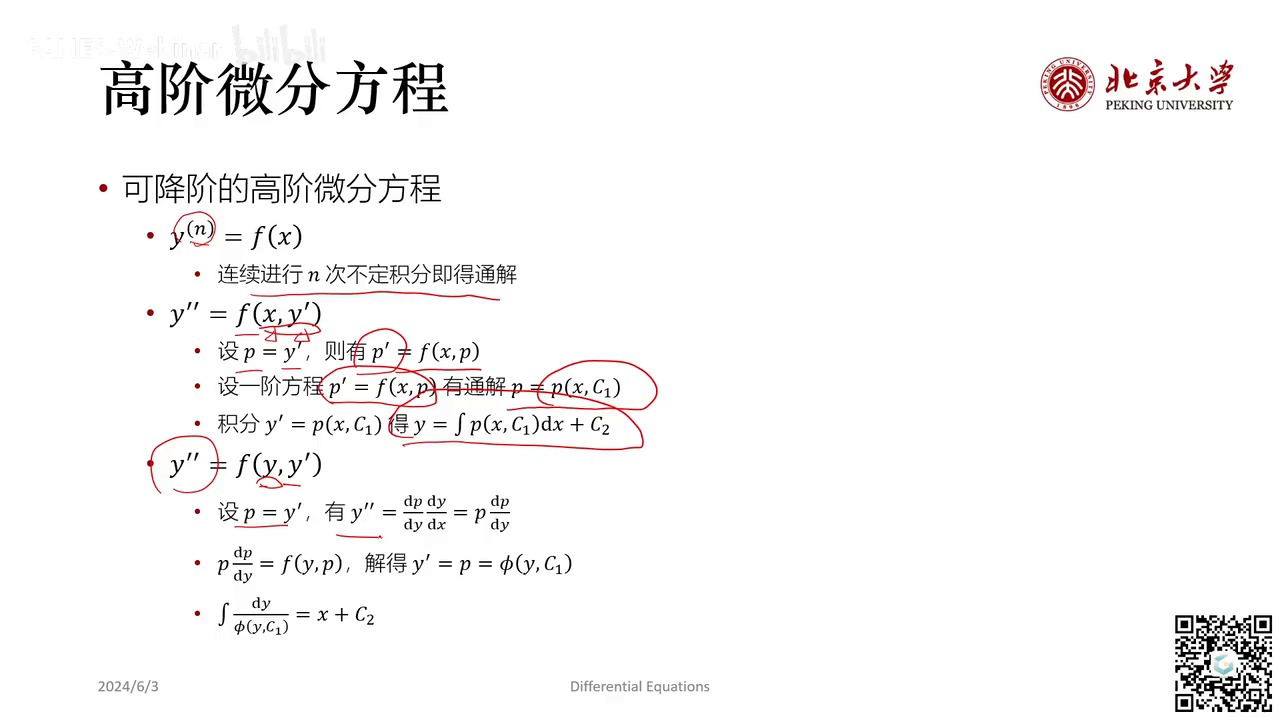
\includegraphics[width=0.92\textwidth]{figures/fig_06_reducible.jpg}
\caption{可降阶的高阶微分方程\vtag}
\end{figure}
\srcnote{00:16:15--00:16:30}
\end{minipage}


前面都是一阶方程，高阶方程最简单的情形是可以降阶的：
\begin{itemize}
\item $y^{(n)}=f(x)$：连续进行 $n$ 次不定积分即得通解。
\item $y''=f(x,y')$：设 $p=y'$，则有 $p'=f(x,p)$；设这个一阶方程有通解 $p=p(x,C_1)$，再积分 $y'=p(x,C_1)$ 得 $y=\int p(x,C_1)\mathrm{d}x+C_2$。
\item $y''=f(y,y')$：设 $p=y'$，有 $y''=\frac{\mathrm{d}p}{\mathrm{d}y}\frac{\mathrm{d}y}{\mathrm{d}x}=p\frac{\mathrm{d}p}{\mathrm{d}y}$，于是 $p\frac{\mathrm{d}p}{\mathrm{d}y}=f(y,p)$，解得 $y'=p=\phi(y,C_1)$，再分离变量 $\int\frac{\mathrm{d}y}{\phi(y,C_1)}=x+C_2$。
\end{itemize}

\section{二阶线性微分方程}

\subsection{解的结构}

\noindent\begin{minipage}{\textwidth}
\begin{figure}[H]
\centering
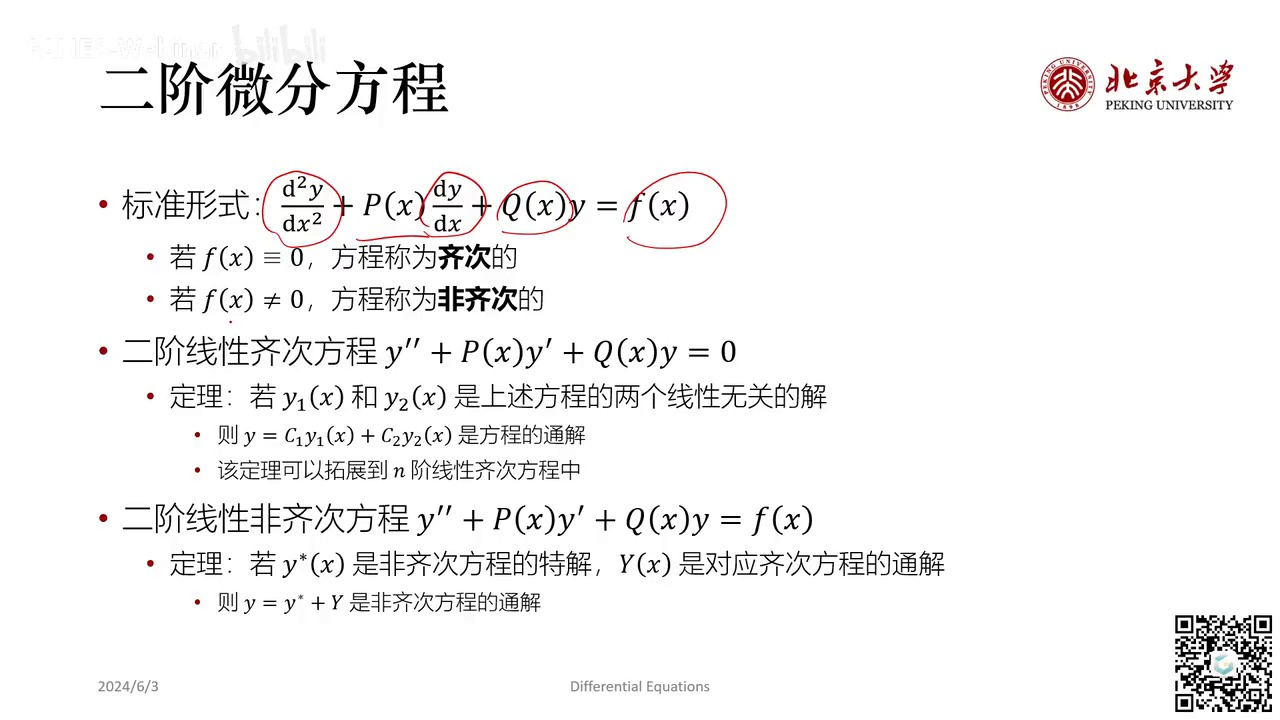
\includegraphics[width=0.92\textwidth]{figures/fig_07_second_order.jpg}
\caption{二阶微分方程的标准形式与解的结构定理\vtag}
\end{figure}
\srcnote{00:17:15--00:17:30}
\end{minipage}


二阶微分方程的标准形式为
\begin{equation}
\frac{\mathrm{d}^2y}{\mathrm{d}x^2}+P(x)\frac{\mathrm{d}y}{\mathrm{d}x}+Q(x)y=f(x).
\end{equation}
若 $f(x)\equiv 0$，方程称为齐次的；否则称为非齐次的。

二阶线性齐次方程 $y''+P(x)y'+Q(x)y=0$ 的定理：若 $y_1(x)$ 和 $y_2(x)$ 是方程的两个线性无关的解，则 $y=C_1y_1(x)+C_2y_2(x)$ 是方程的通解。该定理可以拓展到 $n$ 阶线性齐次方程中。讲者强调，只要找到两个线性无关的特解，它们的线性组合就是通解。

二阶线性非齐次方程 $y''+P(x)y'+Q(x)y=f(x)$ 的定理：若 $y^*(x)$ 是非齐次方程的特解，$Y(x)$ 是对应齐次方程的通解，则 $y=y^*+Y$ 是非齐次方程的通解。

\subsection{二阶常系数齐次线性方程}

\noindent\begin{minipage}{\textwidth}
\begin{figure}[H]
\centering
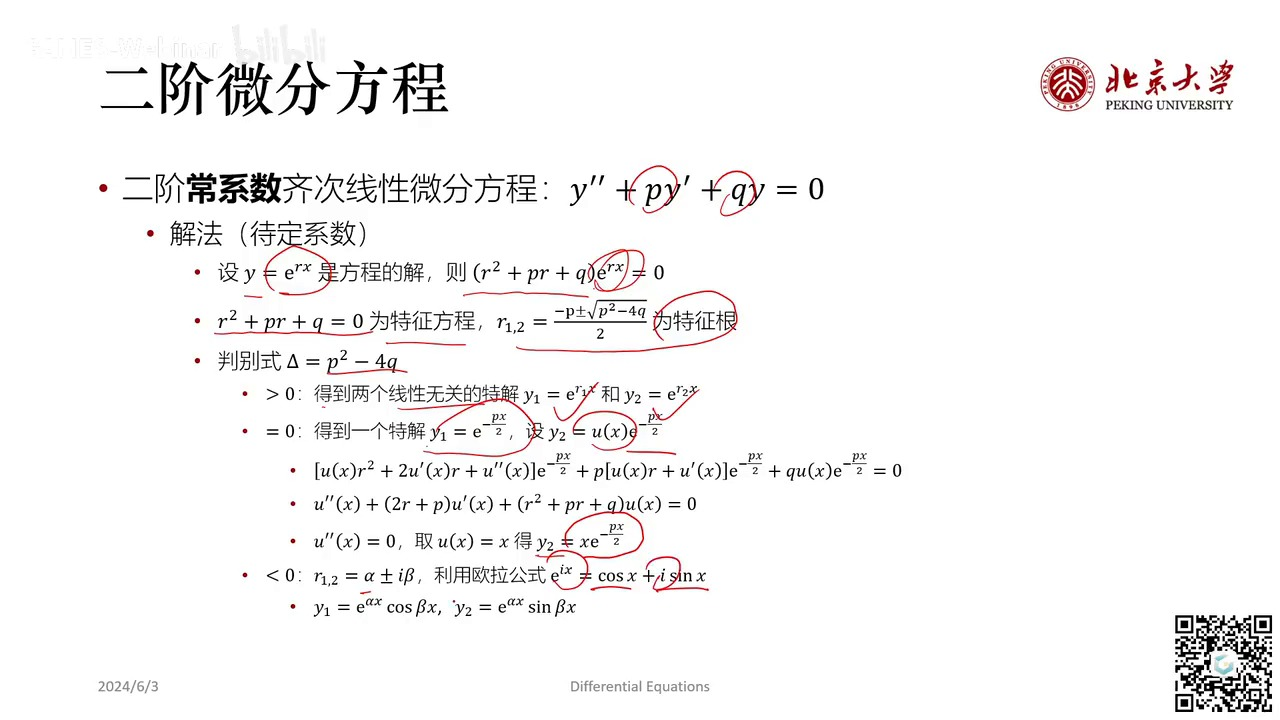
\includegraphics[width=0.92\textwidth]{figures/fig_08_constant_coeff.jpg}
\caption{二阶常系数齐次线性微分方程的解法\vtag}
\end{figure}
\srcnote{00:20:45--00:21:00}
\end{minipage}


对二阶常系数齐次线性方程 $y''+py'+qy=0$，用待定系数法：设 $y=e^{rx}$ 是方程的解。讲者解释为什么这样猜：$e^{rx}$ 不管求多少次导数都会保留因子 $e^{rx}$，这个性质很好。代入得 $(r^2+pr+q)e^{rx}=0$，所以
\begin{equation}
r^2+pr+q=0
\end{equation}
称为特征方程，$r_{1,2}=\frac{-p\pm\sqrt{p^2-4q}}{2}$ 为特征根。看判别式 $\Delta=p^2-4q$：
\begin{itemize}
\item $\Delta>0$：得到两个线性无关的特解 $y_1=e^{r_1x}$ 和 $y_2=e^{r_2x}$。
\item $\Delta=0$：只得到一个特解 $y_1=e^{-\frac{p}{2}x}$。还想找另一个，就依然去猜：设 $y_2=u(x)e^{-\frac{p}{2}x}$，代入整理得 $u''(x)+(2r+p)u'(x)+(r^2+pr+q)u(x)=0$，后两项系数都为零，所以 $u''(x)=0$，取 $u(x)=x$，得 $y_2=xe^{-\frac{p}{2}x}$。
\item $\Delta<0$：$r_{1,2}=\alpha\pm i\beta$，利用欧拉公式 $e^{ix}=\cos x+i\sin x$，取实部和虚部，得 $y_1=e^{\alpha x}\cos\beta x$，$y_2=e^{\alpha x}\sin\beta x$。
\end{itemize}

\begin{practicebox}{用阻尼振子检验三种情形}
讲义作者补充：弹簧阻尼系统 $y''+2\zeta\omega y'+\omega^2y=0$ 的判别式为 $4\omega^2(\zeta^2-1)$。读者可以验证：$\zeta>1$ 时两个实根，物体缓慢回到平衡位置（过阻尼）；$\zeta=1$ 时重根，解为 $(C_1+C_2x)e^{-\omega x}$，回到平衡最快且不振荡（临界阻尼）；$\zeta<1$ 时复根，解为衰减的正弦振荡（欠阻尼）。物理模拟中调弹簧参数时，常以临界阻尼为参照。
\end{practicebox}

\subsection{高阶常系数与非齐次情形}

\noindent\begin{minipage}{\textwidth}
\begin{figure}[H]
\centering
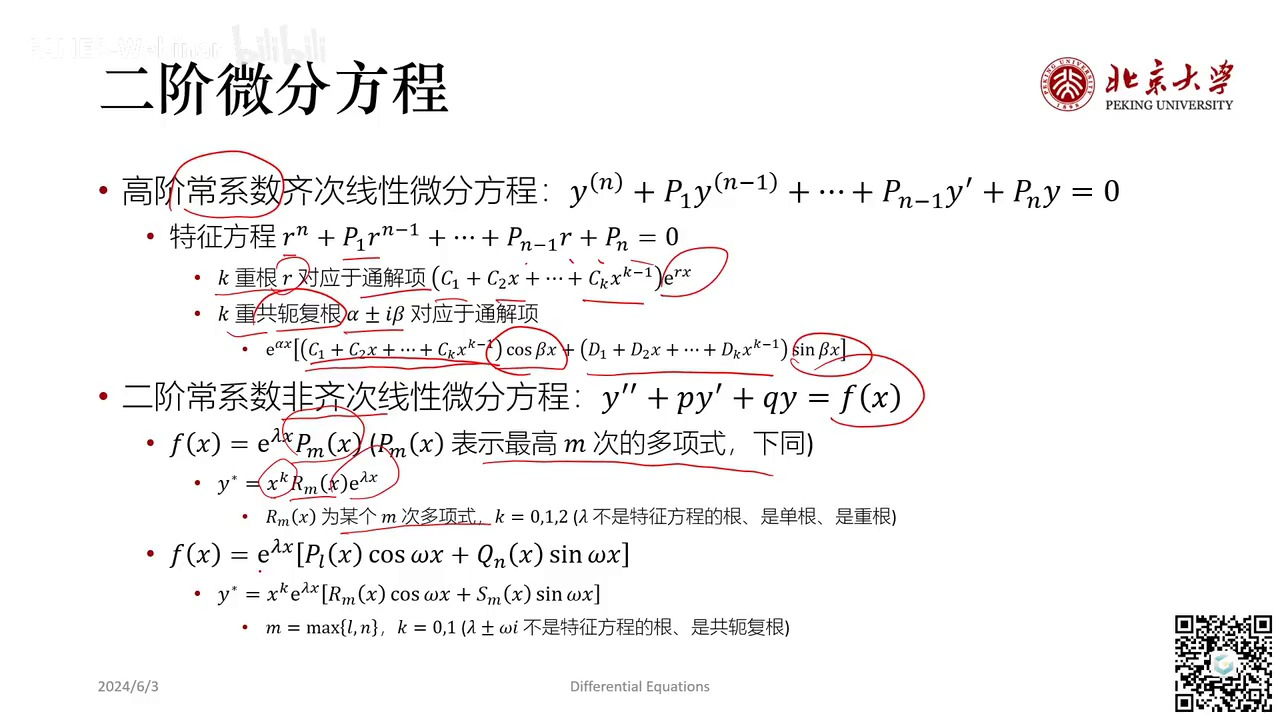
\includegraphics[width=0.92\textwidth]{figures/fig_09_higher_constant.jpg}
\caption{高阶常系数齐次方程与二阶常系数非齐次方程的特解形式\vtag}
\end{figure}
\srcnote{00:22:45--00:23:00}
\end{minipage}


上述论证可以扩展到高阶常系数齐次线性方程 $y^{(n)}+P_1y^{(n-1)}+\cdots+P_{n-1}y'+P_ny=0$：解特征方程
\begin{equation}
r^n+P_1r^{n-1}+\cdots+P_{n-1}r+P_n=0 .
\end{equation}
$k$ 重根 $r$ 对应于通解项 $(C_1+C_2x+\cdots+C_kx^{k-1})e^{rx}$；$k$ 重共轭复根 $\alpha\pm i\beta$ 对应于通解项 $e^{\alpha x}\big[(C_1+C_2x+\cdots+C_kx^{k-1})\cos\beta x+(D_1+D_2x+\cdots+D_kx^{k-1})\sin\beta x\big]$。

二阶常系数非齐次线性方程 $y''+py'+qy=f(x)$ 的特解，根据右端 $f(x)$ 的形式来猜：
\begin{itemize}
\item $f(x)=e^{\lambda x}P_m(x)$，$P_m$ 表示最高 $m$ 次的多项式：特解为 $y^*=x^kR_m(x)e^{\lambda x}$，$R_m(x)$ 为某个 $m$ 次多项式，$k=0,1,2$ 分别对应 $\lambda$ 不是特征方程的根、是单根、是重根。
\item $f(x)=e^{\lambda x}[P_l(x)\cos\omega x+Q_n(x)\sin\omega x]$：特解为 $y^*=x^ke^{\lambda x}[R_m(x)\cos\omega x+S_m(x)\sin\omega x]$，其中 $m=\max\{l,n\}$，$k=0,1$ 分别对应 $\lambda\pm\omega i$ 不是特征方程的根、是共轭复根。
\end{itemize}

\section{二阶偏微分方程}

\subsection{分类}

\noindent\begin{minipage}{\textwidth}
\begin{figure}[H]
\centering
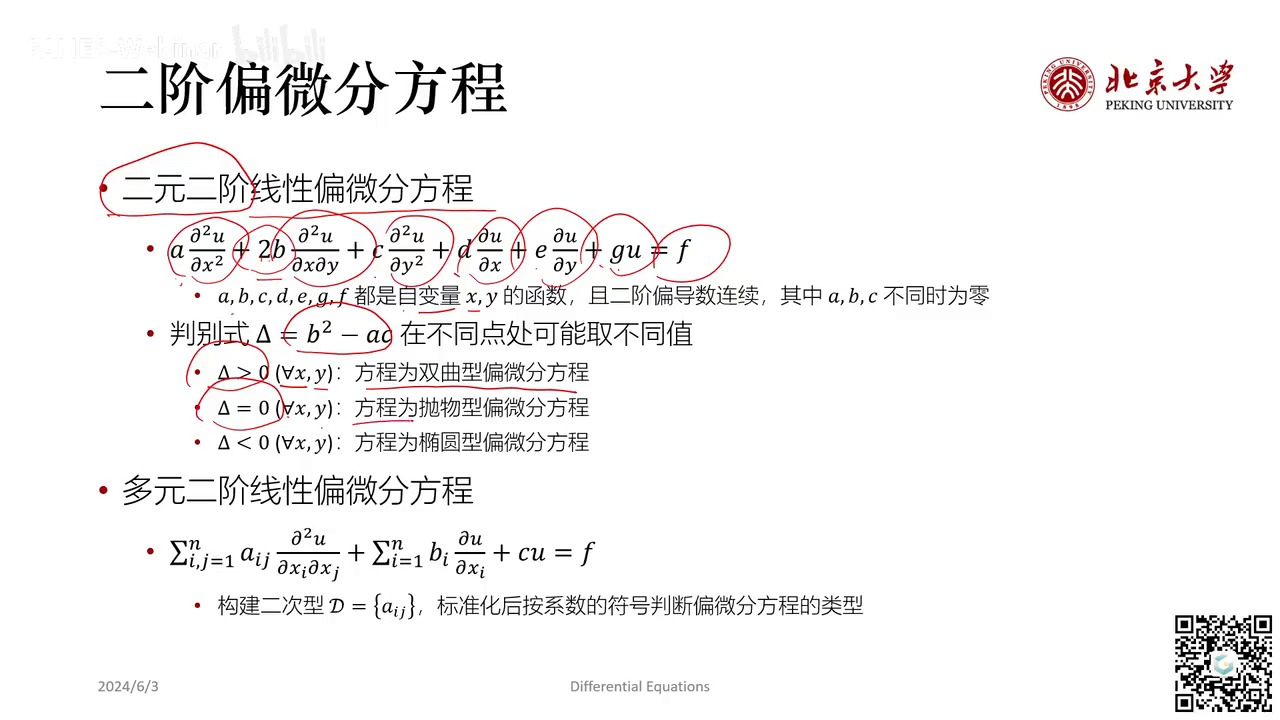
\includegraphics[width=0.92\textwidth]{figures/fig_10_pde_class.jpg}
\caption{二元二阶线性偏微分方程及其分类\vtag}
\end{figure}
\srcnote{00:25:15--00:25:30}
\end{minipage}


讲者说，从这一部分开始，相对来说需要更专业的数学基础。二元二阶线性偏微分方程为
\begin{equation}
a\frac{\partial^2u}{\partial x^2}+2b\frac{\partial^2u}{\partial x\partial y}+c\frac{\partial^2u}{\partial y^2}+d\frac{\partial u}{\partial x}+e\frac{\partial u}{\partial y}+gu=f,
\end{equation}
其中 $a,b,c,d,e,g,f$ 都是自变量 $x,y$ 的函数，且二阶偏导数连续，$a,b,c$ 不同时为零。系数里写成 $2b$，是为了让判别式的形式更简洁。判别式 $\Delta=b^2-ac$ 在不同点处可能取不同值：
\begin{itemize}
\item $\Delta>0\ (\forall x,y)$：方程为双曲型偏微分方程；
\item $\Delta=0\ (\forall x,y)$：方程为抛物型偏微分方程；
\item $\Delta<0\ (\forall x,y)$：方程为椭圆型偏微分方程。
\end{itemize}
讲者解释，把二阶项看成二次型，它就是一个圆锥曲线的标准形式，所以这里的命名来自圆锥曲线。

多元二阶线性偏微分方程 $\sum_{i,j=1}^{n}a_{ij}\frac{\partial^2u}{\partial x_i\partial x_j}+\sum_{i=1}^{n}b_i\frac{\partial u}{\partial x_i}+cu=f$ 也类似：构建二次型 $D=\{a_{ij}\}$，标准化后按系数的符号判断偏微分方程的类型。

\subsection{三个典型方程}

\noindent\begin{minipage}{\textwidth}
\begin{figure}[H]
\centering
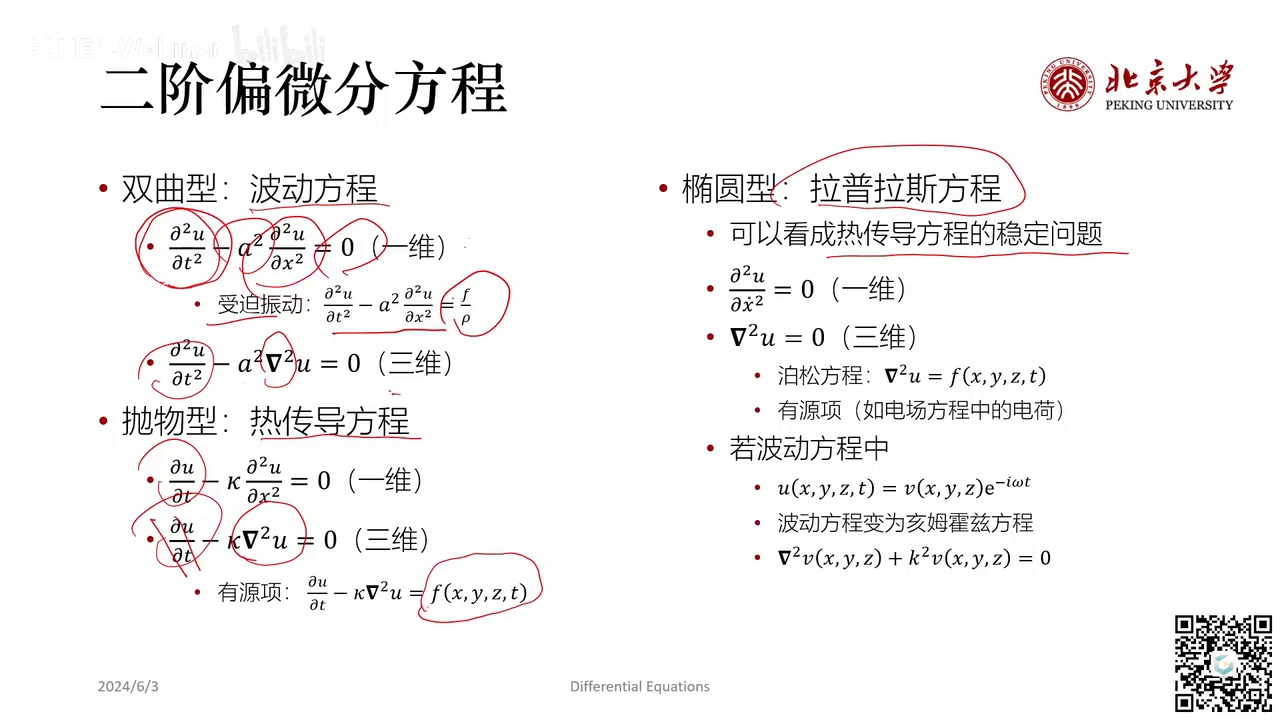
\includegraphics[width=0.92\textwidth]{figures/fig_11_pde_examples.jpg}
\caption{波动方程、热传导方程与拉普拉斯方程\vtag}
\end{figure}
\srcnote{00:29:15--00:29:30}
\end{minipage}


\textbf{双曲型：波动方程。}有两个自变量，时间 $t$ 和位置 $x$，一维振动满足
\begin{equation}
\frac{\partial^2u}{\partial t^2}-a^2\frac{\partial^2u}{\partial x^2}=0\quad(\text{一维}),\qquad \frac{\partial^2u}{\partial t^2}-a^2\nabla^2u=0\quad(\text{三维}).
\end{equation}
受迫振动时右端有外力项 $f/\rho$。

\textbf{抛物型：热传导方程。}
\begin{equation}
\frac{\partial u}{\partial t}-\kappa\frac{\partial^2u}{\partial x^2}=0\quad(\text{一维}),\qquad \frac{\partial u}{\partial t}-\kappa\nabla^2u=0\quad(\text{三维}),
\end{equation}
有源项时右端为 $f(x,y,z,t)$。讲者让大家比较它和波动方程的区别：主要区别在关于时间 $t$ 的那一项，波动方程对 $t$ 求二阶偏导，热传导方程只求一阶。

\textbf{椭圆型：拉普拉斯方程。}它可以看成热传导方程的稳定问题。讲者的解释是：假如不停地传热，最后空间会形成稳定的热分布，对时间的导数项就消失了，剩下 $\frac{\partial^2u}{\partial x^2}=0$（一维）或 $\nabla^2u=0$（三维），这就是拉普拉斯方程。有源项时为泊松方程 $\nabla^2u=f(x,y,z,t)$，比如电场方程中的电荷。

若波动方程中 $u(x,y,z,t)=v(x,y,z)e^{-i\omega t}$，代入后波动方程变为亥姆霍兹方程
\begin{equation}
\nabla^2v(x,y,z)+k^2v(x,y,z)=0 .
\end{equation}

\begin{knowledgebox}{三类方程的物理直觉}
讲义作者补充：双曲型方程描述“传播”，扰动以有限速度传出去，能量守恒，如声波和弦振动；抛物型方程描述“扩散”，扰动瞬间影响各处但迅速平滑，如热传导与图像的高斯模糊；椭圆型方程描述“平衡”，解由边界条件整体决定，如稳态温度和静电势。图形学中，布料和流体中会遇到双曲型与抛物型，网格平滑、参数化、泊松图像编辑则大多是椭圆型。
\end{knowledgebox}

\section{分离变量法}

\subsection{波动方程的分离变量}

\noindent\begin{minipage}{\textwidth}
\begin{figure}[H]
\centering
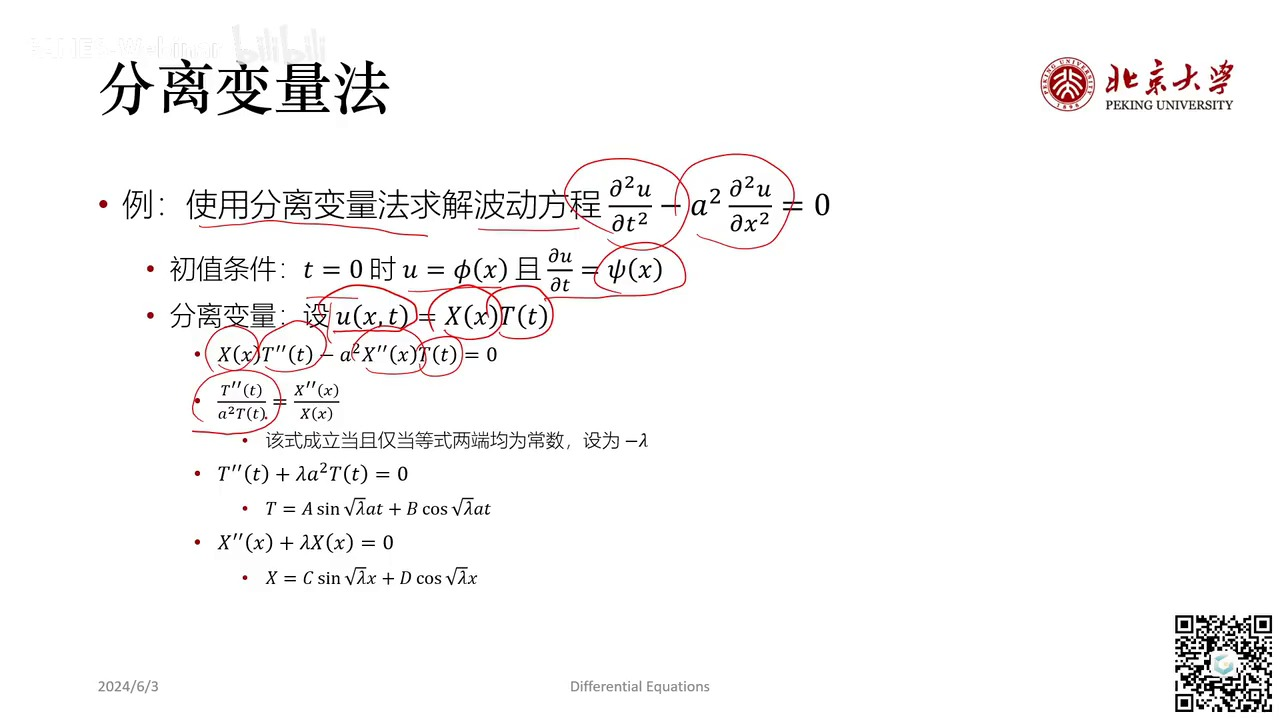
\includegraphics[width=0.92\textwidth]{figures/fig_12_sepvar1.jpg}
\caption{用分离变量法求解一维波动方程\vtag}
\end{figure}
\srcnote{00:31:30--00:31:45}
\end{minipage}


例：使用分离变量法求解波动方程 $\frac{\partial^2u}{\partial t^2}-a^2\frac{\partial^2u}{\partial x^2}=0$，初值条件：$t=0$ 时 $u=\phi(x)$ 且 $\frac{\partial u}{\partial t}=\psi(x)$。

假设 $u(x,t)$ 中 $x$ 和 $t$ 是可分离的，即等于关于 $x$ 的函数与关于 $t$ 的函数相乘，$u(x,t)=X(x)T(t)$。代入得 $X(x)T''(t)-a^2X''(x)T(t)=0$，即
\begin{equation}
\frac{T''(t)}{a^2T(t)}=\frac{X''(x)}{X(x)}.
\end{equation}
左边只与 $t$ 有关，右边只与 $x$ 有关，该式成立当且仅当等式两端均为常数，设为 $-\lambda$。于是得到两个二阶线性齐次常微分方程：
\begin{equation}
T''(t)+\lambda a^2T(t)=0,\qquad X''(x)+\lambda X(x)=0,
\end{equation}
解得 $T=A\sin\sqrt\lambda at+B\cos\sqrt\lambda at$，$X=C\sin\sqrt\lambda x+D\cos\sqrt\lambda x$。

\subsection{加上边界条件}

\noindent\begin{minipage}{\textwidth}
\begin{figure}[H]
\centering
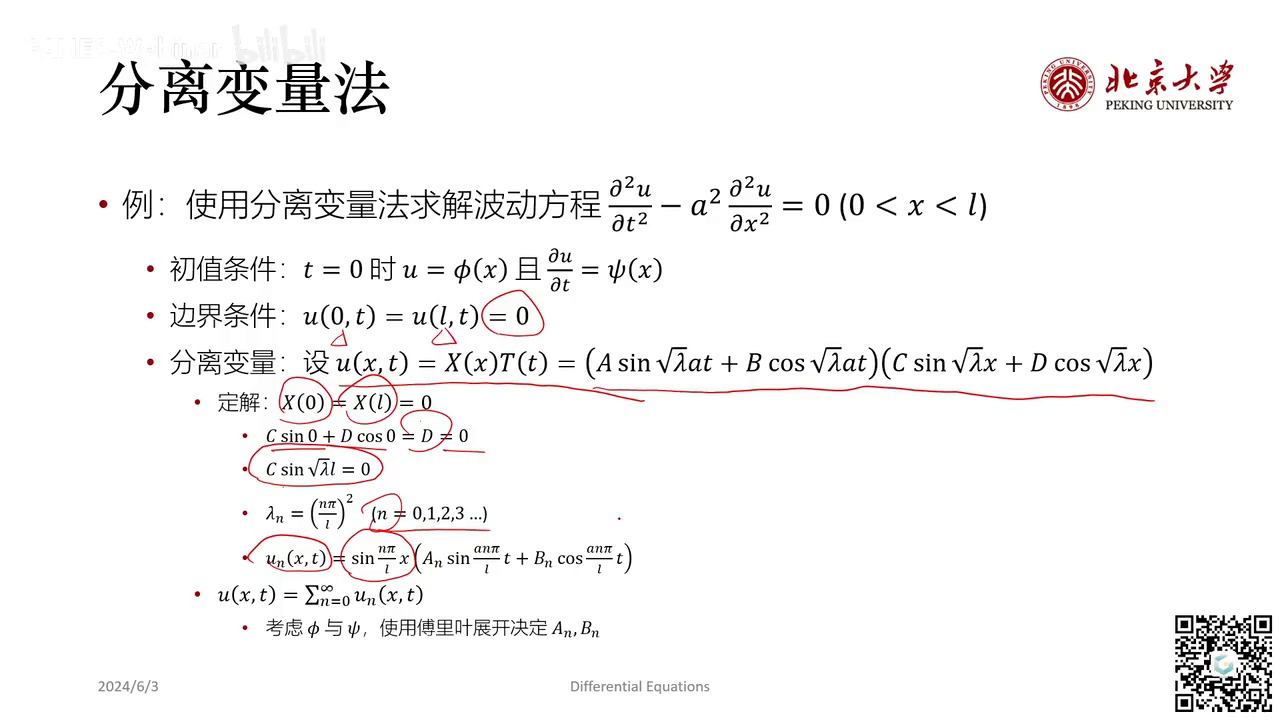
\includegraphics[width=0.92\textwidth]{figures/fig_13_sepvar2.jpg}
\caption{加上边界条件后的定解与傅里叶展开\vtag}
\end{figure}
\srcnote{00:34:15--00:34:30}
\end{minipage}


再加上边界条件 $u(0,t)=u(l,t)=0$（$0<x<l$）。讲者说，这相当于把弦的两端捏住：在任意时刻，$x=0$ 和 $x=l$ 两个点的位移都不发生改变。由 $X(0)=X(l)=0$：$C\sin 0+D\cos 0=0$ 得 $D=0$；$C\sin\sqrt\lambda l=0$ 要求
\begin{equation}
\lambda_n=\left(\frac{n\pi}{l}\right)^2\qquad(n=0,1,2,3,\dots).
\end{equation}
把 $n$ 作为参量，得到第 $n$ 个分离变量解
\begin{equation}
u_n(x,t)=\sin\frac{n\pi}{l}x\left(A_n\sin\frac{an\pi}{l}t+B_n\cos\frac{an\pi}{l}t\right),
\end{equation}
叠加得 $u(x,t)=\sum_{n=0}^{\infty}u_n(x,t)$。最后考虑初值 $\phi$ 与 $\psi$，用傅里叶展开决定 $A_n,B_n$。

\begin{knowledgebox}{分离变量法的本质}
讲者指出，分离变量法的思想就是傅里叶展开：它给出的是偏微分方程在傅里叶展开形式下的解。讲义作者补充：每个 $u_n$ 是弦的一个“驻波模态”，频率为 $an/(2l)$；边界条件挑出了允许的频率，初值条件决定了每个模态的振幅。这和第七讲“换一组基表示函数”的思想完全一致。
\end{knowledgebox}

\section{球谐函数}

讲者说，在本系列课程中大家可能已经接触到球谐函数了，这里就稍微详细地说明一下：球谐函数来自于拉普拉斯方程。在直角坐标系下分离变量很简单，但在球坐标系下解拉普拉斯方程就比较麻烦，因为三个坐标 $r,\theta,\phi$ 不是对称的。

\subsection{球坐标系下的分离变量}

\noindent\begin{minipage}{\textwidth}
\begin{figure}[H]
\centering
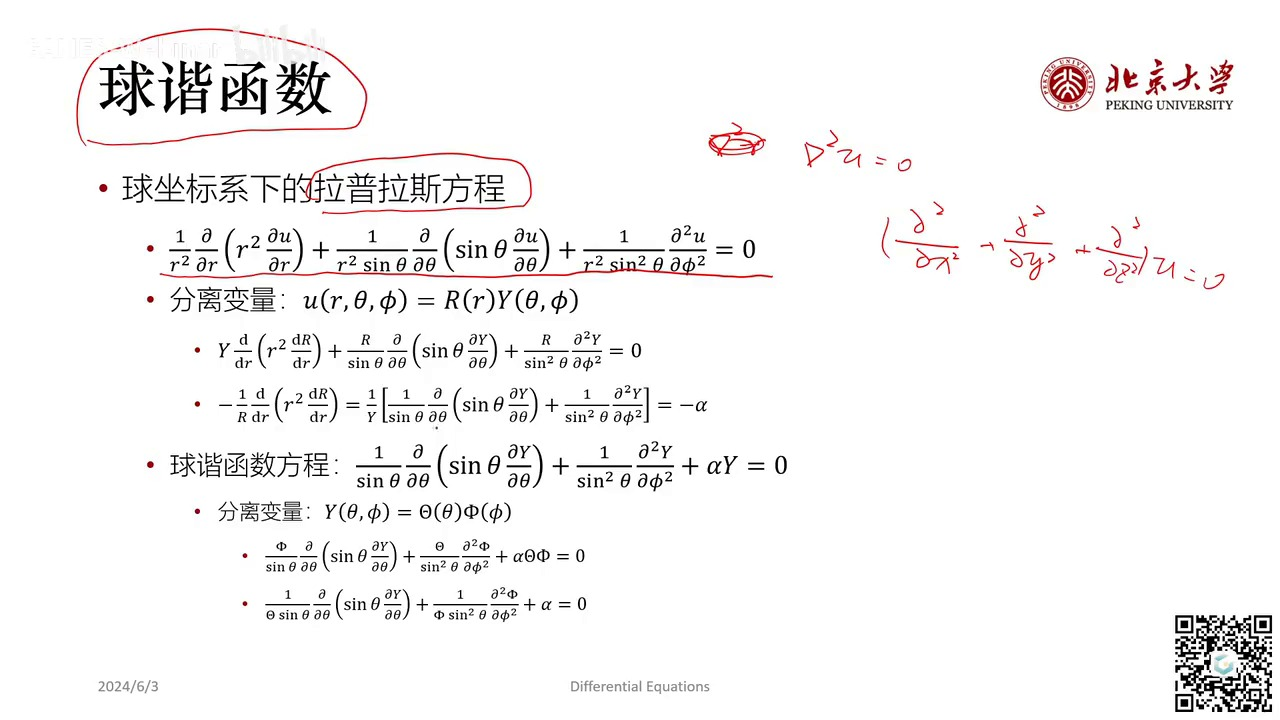
\includegraphics[width=0.92\textwidth]{figures/fig_14_sh_laplace.jpg}
\caption{球坐标系下的拉普拉斯方程与第一次分离变量\vtag}
\end{figure}
\srcnote{00:36:15--00:36:30}
\end{minipage}


球坐标系下的拉普拉斯方程为
\begin{equation}
\frac{1}{r^2}\frac{\partial}{\partial r}\left(r^2\frac{\partial u}{\partial r}\right)+\frac{1}{r^2\sin\theta}\frac{\partial}{\partial\theta}\left(\sin\theta\frac{\partial u}{\partial\theta}\right)+\frac{1}{r^2\sin^2\theta}\frac{\partial^2u}{\partial\phi^2}=0 .
\end{equation}
先分离径向：设 $u(r,\theta,\phi)=R(r)Y(\theta,\phi)$，代入后两边同乘 $r^2/(RY)$，得
\begin{equation}
\frac{1}{R}\frac{\mathrm{d}}{\mathrm{d}r}\left(r^2\frac{\mathrm{d}R}{\mathrm{d}r}\right)=-\frac{1}{Y}\left[\frac{1}{\sin\theta}\frac{\partial}{\partial\theta}\left(\sin\theta\frac{\partial Y}{\partial\theta}\right)+\frac{1}{\sin^2\theta}\frac{\partial^2Y}{\partial\phi^2}\right]=\alpha .
\end{equation}
左右两边分别只与 $r$ 和 $(\theta,\phi)$ 有关，要时刻相等只能等于常数，设为 $\alpha$（课件中记右侧为 $-\alpha$）。由此得到球谐函数方程
\begin{equation}
\frac{1}{\sin\theta}\frac{\partial}{\partial\theta}\left(\sin\theta\frac{\partial Y}{\partial\theta}\right)+\frac{1}{\sin^2\theta}\frac{\partial^2Y}{\partial\phi^2}+\alpha Y=0,
\end{equation}
把方程解出来得到的函数 $Y$ 就叫做球谐函数。

\subsection{再次分离变量}

\noindent\begin{minipage}{\textwidth}
\begin{figure}[H]
\centering
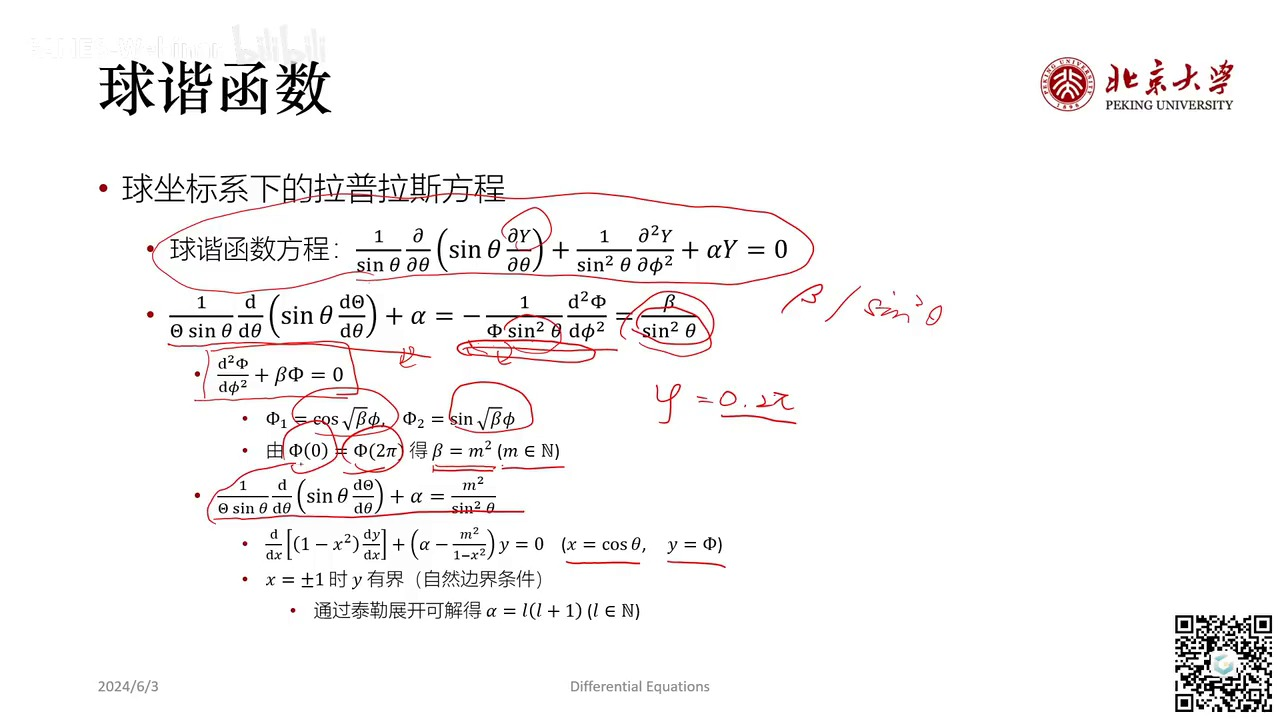
\includegraphics[width=0.92\textwidth]{figures/fig_15_sh_separate.jpg}
\caption{球谐函数方程的再次分离变量与连带勒让德方程\vtag}
\end{figure}
\srcnote{00:40:15--00:40:30}
\end{minipage}


对 $Y$ 再分离变量：$Y(\theta,\phi)=\Theta(\theta)\Phi(\phi)$。代入并乘以 $\sin^2\theta/(\Theta\Phi)$，等式右端所有与 $\sin^2\theta$ 有关的量都可以消掉，得
\begin{equation}
\frac{\sin\theta}{\Theta}\frac{\mathrm{d}}{\mathrm{d}\theta}\left(\sin\theta\frac{\mathrm{d}\Theta}{\mathrm{d}\theta}\right)+\alpha\sin^2\theta=-\frac{1}{\Phi}\frac{\mathrm{d}^2\Phi}{\mathrm{d}\phi^2}=\beta .
\end{equation}
对 $\phi$：$\frac{\mathrm{d}^2\Phi}{\mathrm{d}\phi^2}+\beta\Phi=0$，解为 $\Phi_1=\cos\sqrt\beta\phi$，$\Phi_2=\sin\sqrt\beta\phi$。由周期性 $\Phi(0)=\Phi(2\pi)$ 得 $\beta=m^2$，$m\in\mathbb N$。

对 $\theta$：令 $x=\cos\theta$，$y=\Theta$，整理得
\begin{equation}
\frac{\mathrm{d}}{\mathrm{d}x}\left[(1-x^2)\frac{\mathrm{d}y}{\mathrm{d}x}\right]+\left(\alpha-\frac{m^2}{1-x^2}\right)y=0 .
\end{equation}
$x=\pm 1$ 时 $y$ 有界（自然边界条件），通过泰勒展开可解得 $\alpha=l(l+1)$，$l\in\mathbb N$。

\subsection{解的结构与归一化}

\noindent\begin{minipage}{\textwidth}
\begin{figure}[H]
\centering
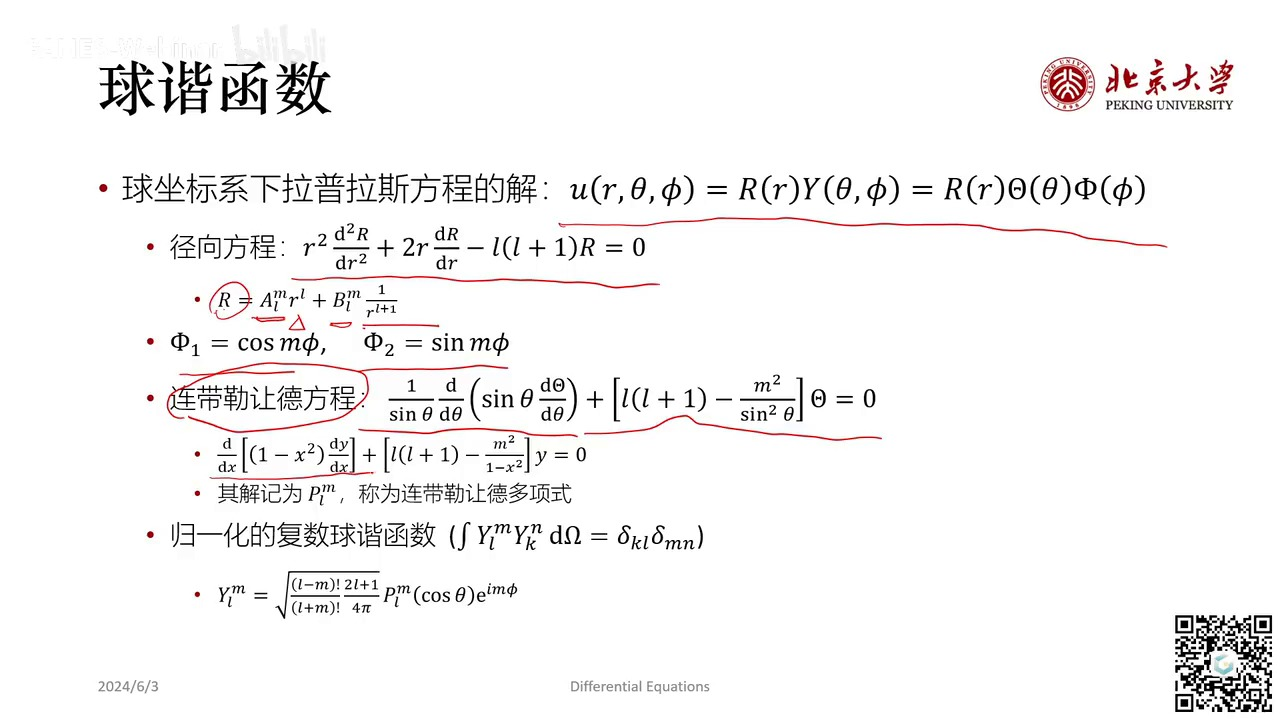
\includegraphics[width=0.92\textwidth]{figures/fig_16_sh_solution.jpg}
\caption{球坐标系下拉普拉斯方程的解：径向方程、连带勒让德方程与复数球谐函数\vtag}
\end{figure}
\srcnote{00:42:30--00:42:45}
\end{minipage}


总之，在球坐标系下解出了拉普拉斯方程的分离变量解 $u(r,\theta,\phi)=R(r)Y(\theta,\phi)=R(r)\Theta(\theta)\Phi(\phi)$：
\begin{itemize}
\item 径向方程 $r^2\frac{\mathrm{d}^2R}{\mathrm{d}r^2}+2r\frac{\mathrm{d}R}{\mathrm{d}r}-l(l+1)R=0$，解为 $R=A_l^mr^l+B_l^m\frac{1}{r^{l+1}}$；
\item $\Phi_1=\cos m\phi$，$\Phi_2=\sin m\phi$；
\item 连带勒让德方程 $\frac{1}{\sin\theta}\frac{\mathrm{d}}{\mathrm{d}\theta}\left(\sin\theta\frac{\mathrm{d}\Theta}{\mathrm{d}\theta}\right)+\left[l(l+1)-\frac{m^2}{\sin^2\theta}\right]\Theta=0$，其解记为 $P_l^m$，称为连带勒让德多项式。
\end{itemize}
在复数域下往往还要求球谐函数是归一化的，$\int Y_l^m\overline{Y_k^n}\,\mathrm{d}\Omega=\delta_{kl}\delta_{mn}$，得到
\begin{equation}
Y_l^m=\sqrt{\frac{(l-m)!}{(l+m)!}\frac{2l+1}{4\pi}}\,P_l^m(\cos\theta)\,e^{im\phi}.
\end{equation}

\subsection{实球谐函数与勒让德多项式}

\noindent\begin{minipage}{\textwidth}
\begin{figure}[H]
\centering
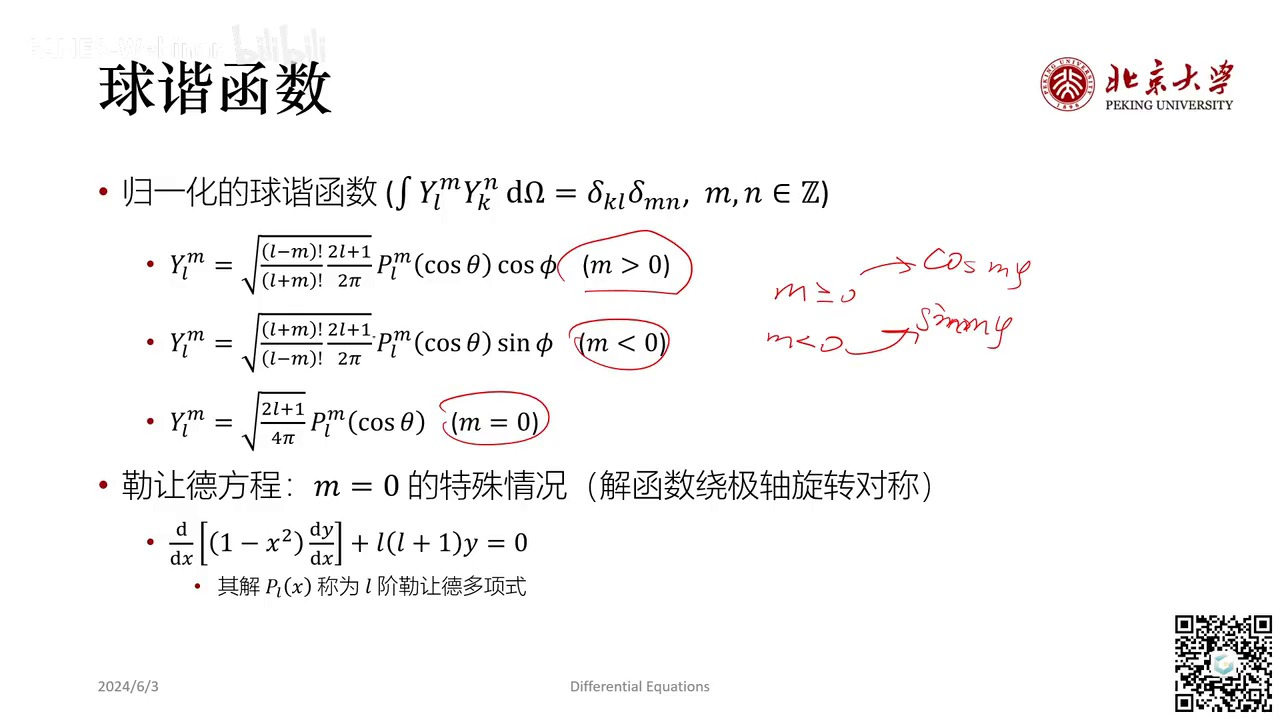
\includegraphics[width=0.92\textwidth]{figures/fig_17_sh_real.jpg}
\caption{归一化的实球谐函数与勒让德方程\vtag}
\end{figure}
\srcnote{00:44:15--00:44:30}
\end{minipage}


讲者说，$\cos m\phi$ 和 $\sin m\phi$ 两种解可以用 $m$ 的正负来区分，把 $m<0$ 的情况也利用起来，得到归一化的实球谐函数（$\int Y_l^mY_k^n\,\mathrm{d}\Omega=\delta_{kl}\delta_{mn}$）：
\begin{equation}
Y_l^m=\begin{cases}
\sqrt{\frac{(l-m)!}{(l+m)!}\frac{2l+1}{2\pi}}\,P_l^m(\cos\theta)\cos m\phi, & m>0,\\[4pt]
\sqrt{\frac{(l-|m|)!}{(l+|m|)!}\frac{2l+1}{2\pi}}\,P_l^{|m|}(\cos\theta)\sin|m|\phi, & m<0,\\[4pt]
\sqrt{\frac{2l+1}{4\pi}}\,P_l^m(\cos\theta), & m=0 .
\end{cases}
\end{equation}

\begin{warningbox}{$m<0$ 时的写法}
课件上 $m<0$ 一行的阶乘和 $P_l^m$ 中直接写的是 $m$。讲义作者按常用约定改为 $|m|$：$m<0$ 时实际使用的是 $P_l^{|m|}$ 和 $\sin|m|\phi$，否则阶乘 $(l+m)!$ 在 $m$ 为负时与归一化条件不符，也不会得到 $m$ 阶的方位变化。
\end{warningbox}

$m=0$ 是一个特殊情况，此时解函数绕极轴旋转对称，与 $\phi$ 无关，不管 $\phi$ 怎么变得到的结果都相同。方程变为勒让德方程
\begin{equation}
\frac{\mathrm{d}}{\mathrm{d}x}\left[(1-x^2)\frac{\mathrm{d}y}{\mathrm{d}x}\right]+l(l+1)y=0,
\end{equation}
其解 $P_l(x)$ 称为 $l$ 阶勒让德多项式。

\subsection{勒让德多项式与应用}

\noindent\begin{minipage}{\textwidth}
\begin{figure}[H]
\centering
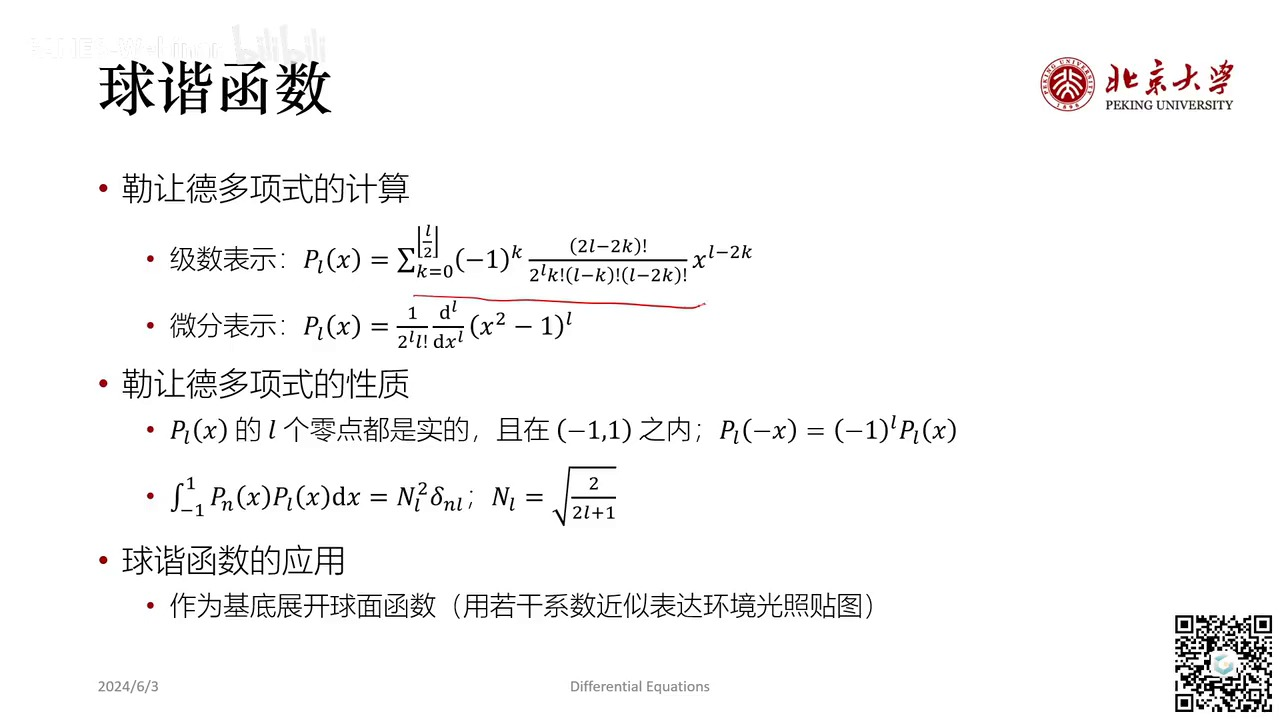
\includegraphics[width=0.92\textwidth]{figures/fig_18_legendre.jpg}
\caption{勒让德多项式的计算、性质与球谐函数的应用\vtag}
\end{figure}
\srcnote{00:45:30--00:45:45}
\end{minipage}


勒让德多项式有两种表示。级数表示为
\begin{equation}
P_l(x)=\sum_{k=0}^{\lfloor l/2\rfloor}(-1)^k\frac{(2l-2k)!}{2^lk!\,(l-k)!\,(l-2k)!}x^{l-2k},
\end{equation}
微分表示为 $P_l(x)=\frac{1}{2^l\,l!}\frac{\mathrm{d}^l}{\mathrm{d}x^l}(x^2-1)^l$。

性质：$P_l(x)$ 的 $l$ 个零点都是实的，且在 $(-1,1)$ 之内；$P_l(-x)=(-1)^lP_l(x)$，即要么是奇函数、要么是偶函数；正交性 $\int_{-1}^{1}P_n(x)P_l(x)\,\mathrm{d}x=N_l^2\delta_{nl}$，$N_l=\sqrt{2/(2l+1)}$。讲者解释：$n$ 和 $l$ 不同时，两个多项式相乘在 $[-1,1]$ 上积分为零。

\noindent\begin{minipage}{\textwidth}
\begin{figure}[H]
\centering
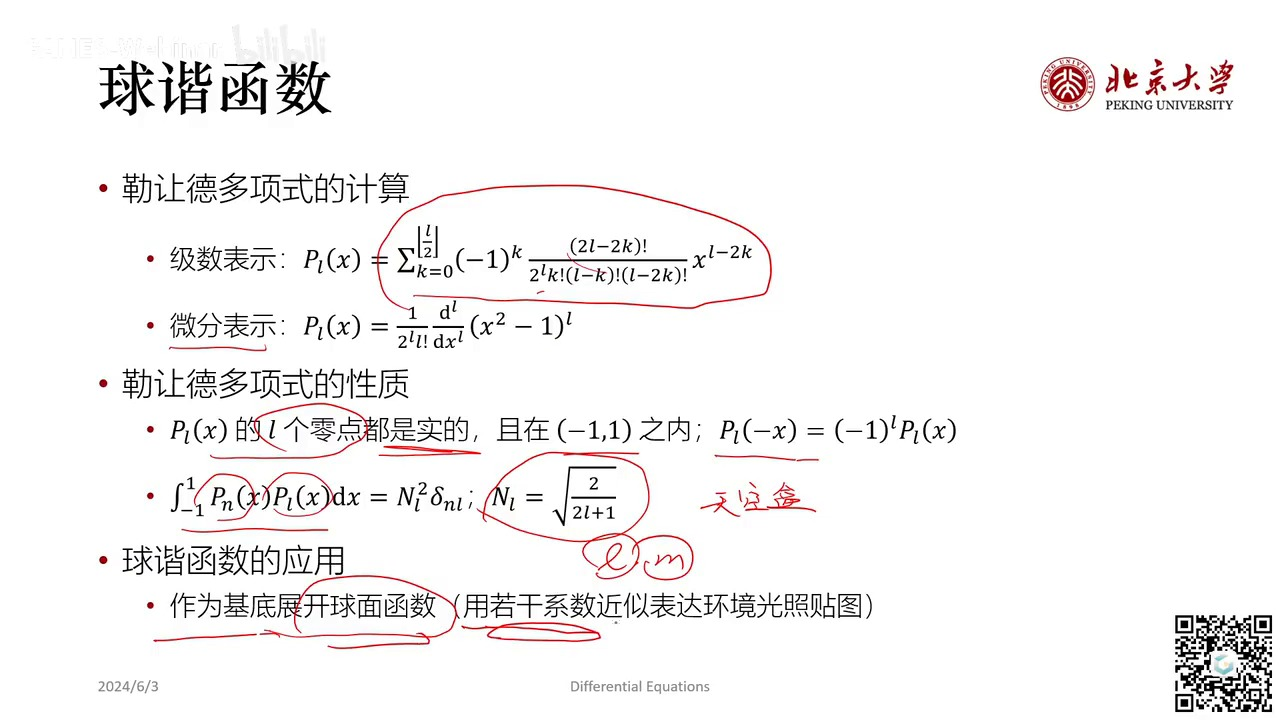
\includegraphics[width=0.92\textwidth]{figures/fig_19_legendre_note.jpg}
\caption{讲者在“用若干系数近似表达环境光照贴图”旁的批注\vtag}
\end{figure}
\srcnote{00:47:30--00:47:45}
\end{minipage}


球谐函数的应用：作为基底展开球面函数，用若干系数近似表达环境光照贴图。讲者解释，环境光照贴图如果直接存储，不仅数据量大，而且使用时要做插值、做寻址，计算量都很大；用球谐函数展开，只取较低阶的 $l$ 和 $m$，就只剩若干个系数，因为球谐函数本身是固定的，每一项只与系数有关。

\section{格林函数法}

\subsection{从电场问题说起}

\noindent\begin{minipage}{\textwidth}
\begin{figure}[H]
\centering
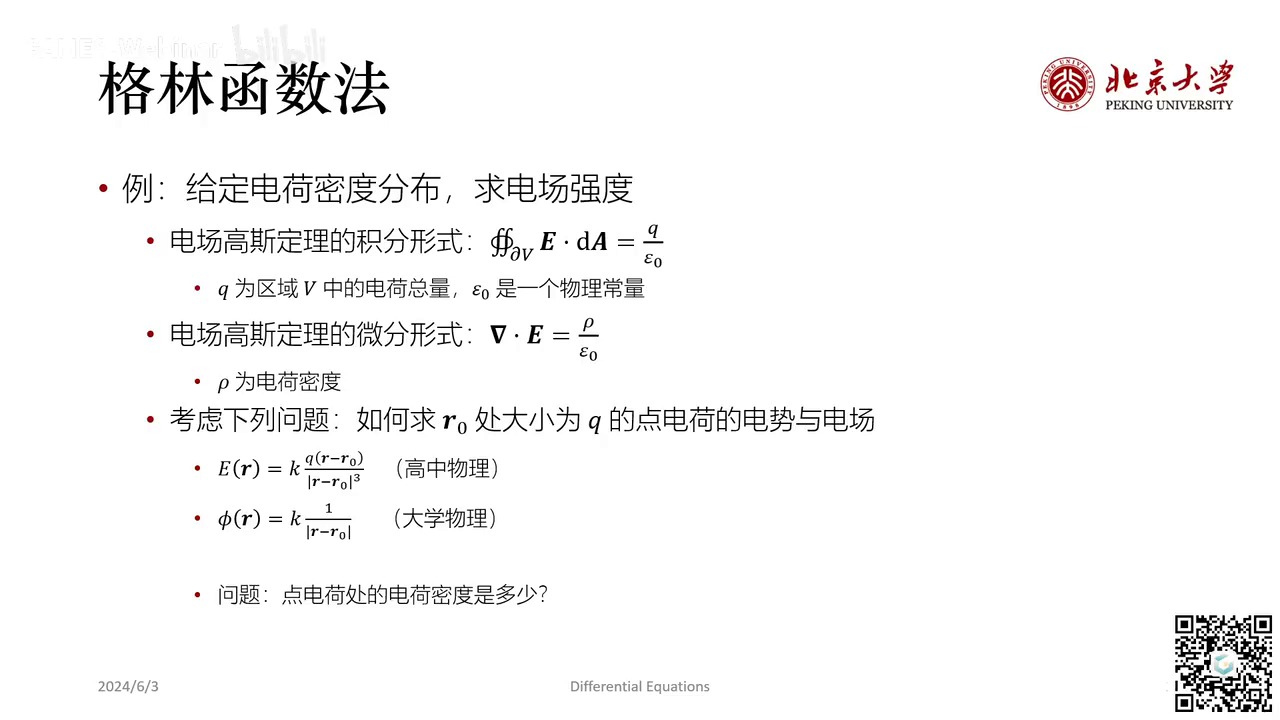
\includegraphics[width=0.92\textwidth]{figures/fig_20_green_intro.jpg}
\caption{格林函数法的引例：给定电荷密度分布求电场强度\vtag}
\end{figure}
\srcnote{00:48:00--00:48:15}
\end{minipage}


例：给定空间中的电荷密度分布，求电场强度。电场高斯定理的积分形式为 $\oint_{\partial V}\boldsymbol E\cdot\mathrm{d}\boldsymbol A=\frac{q}{\varepsilon_0}$，$q$ 为区域 $V$ 中的电荷总量，$\varepsilon_0$ 是一个物理常量；微分形式为 $\nabla\cdot\boldsymbol E=\frac{\rho}{\varepsilon_0}$，$\rho$ 为电荷密度。

考虑下列问题：如何求 $\boldsymbol r_0$ 处大小为 $q$ 的点电荷的电势与电场？高中物理告诉我们 $\boldsymbol E(\boldsymbol r)=k\frac{q(\boldsymbol r-\boldsymbol r_0)}{|\boldsymbol r-\boldsymbol r_0|^3}$，大学物理告诉我们 $\phi(\boldsymbol r)=k\frac{q}{|\boldsymbol r-\boldsymbol r_0|}$。讲者说，积分形式还好办，只要把点电荷包起来算面积分就可以了；但如果用微分形式，点电荷附近会发生什么？点电荷处的电荷密度是多少？

\subsection{狄拉克函数}

\noindent\begin{minipage}{\textwidth}
\begin{figure}[H]
\centering
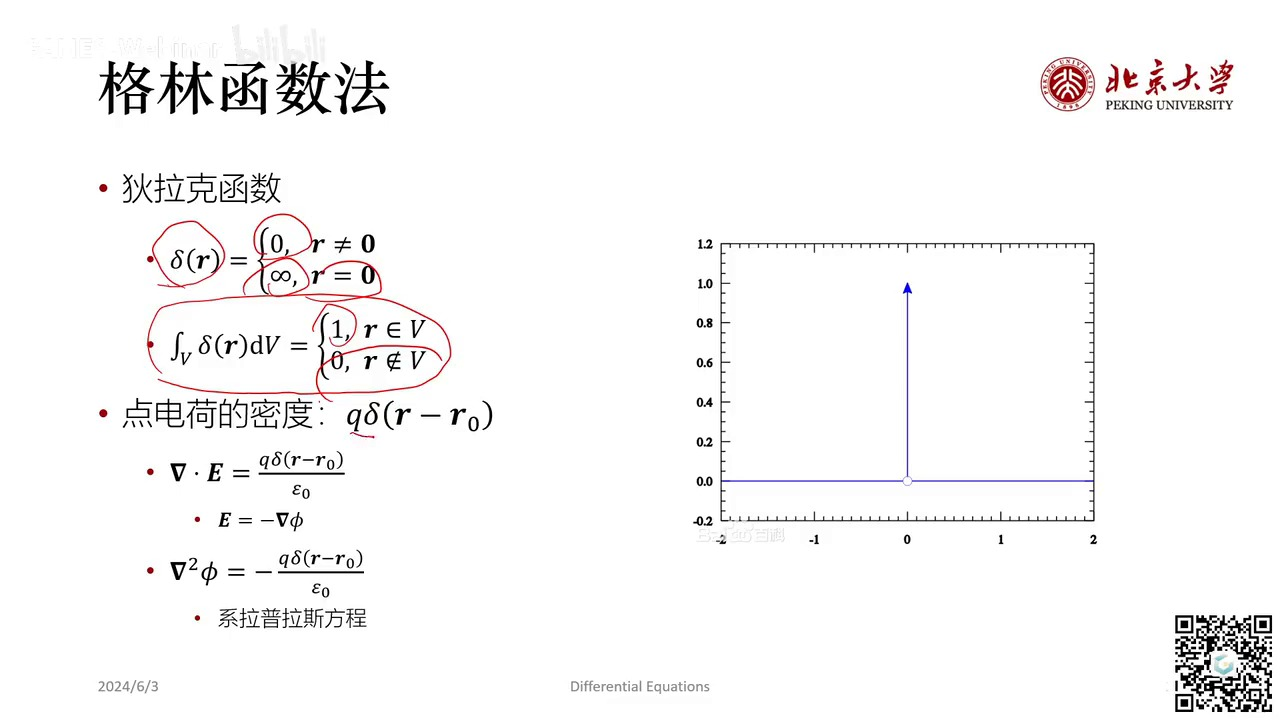
\includegraphics[width=0.92\textwidth]{figures/fig_21_dirac.jpg}
\caption{狄拉克函数与点电荷的密度\vtag}
\end{figure}
\srcnote{00:51:45--00:52:00}
\end{minipage}


这就需要狄拉克函数。在三维中，
\begin{equation}
\delta(\boldsymbol r)=\begin{cases}0,&\boldsymbol r\ne\boldsymbol 0,\\ \infty,&\boldsymbol r=\boldsymbol 0,\end{cases}\qquad \int_V\delta(\boldsymbol r)\,\mathrm{d}V=\begin{cases}1,&\boldsymbol 0\in V,\\0,&\boldsymbol 0\notin V.\end{cases}
\end{equation}
于是点电荷的密度可以写成 $q\delta(\boldsymbol r-\boldsymbol r_0)$，有 $\nabla\cdot\boldsymbol E=\frac{q\delta(\boldsymbol r-\boldsymbol r_0)}{\varepsilon_0}$。令 $\boldsymbol E=-\nabla\phi$，即电场是某个标量势的负梯度，就得到
\begin{equation}
\nabla^2\phi=-\frac{q\delta(\boldsymbol r-\boldsymbol r_0)}{\varepsilon_0},
\end{equation}
这是泊松方程。

\subsection{泊松方程的格林函数解}

\noindent\begin{minipage}{\textwidth}
\begin{figure}[H]
\centering
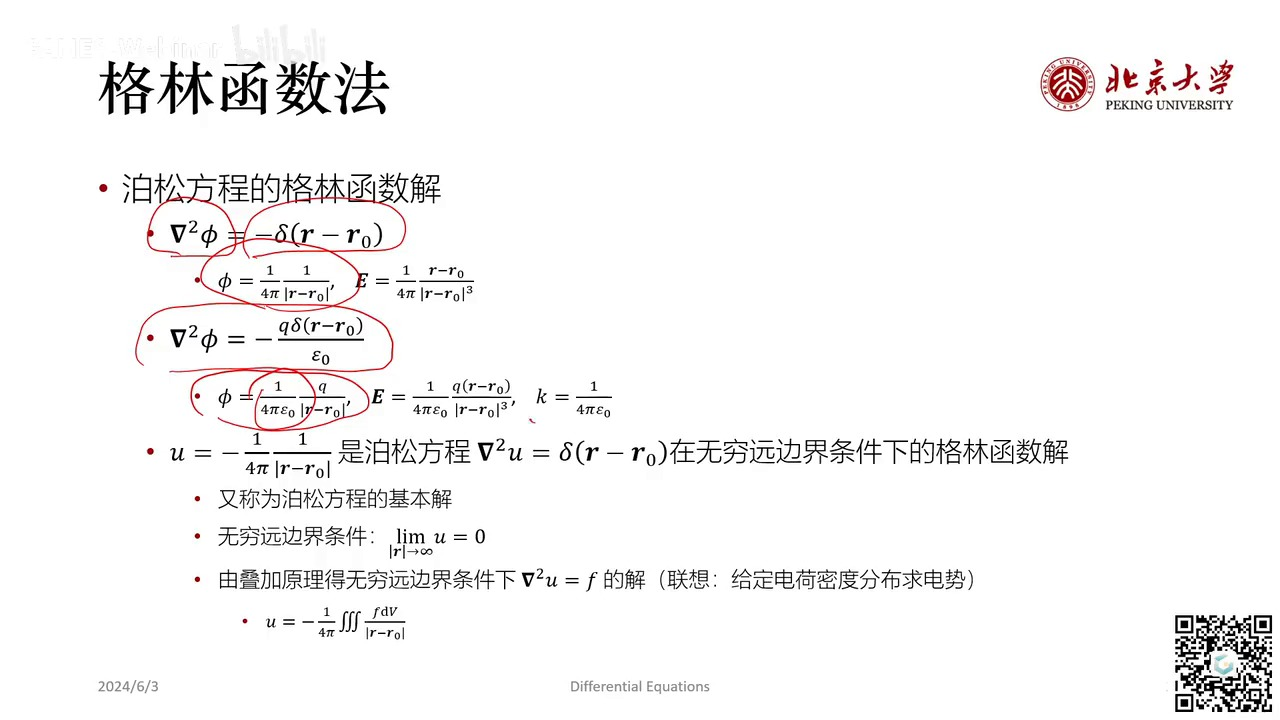
\includegraphics[width=0.92\textwidth]{figures/fig_22_green_poisson.jpg}
\caption{泊松方程的格林函数解：基本解与叠加原理\vtag}
\end{figure}
\srcnote{00:53:15--00:53:30}
\end{minipage}


对 $\nabla^2\phi=-\delta(\boldsymbol r-\boldsymbol r_0)$，解为 $\phi=\frac{1}{4\pi}\frac{1}{|\boldsymbol r-\boldsymbol r_0|}$；对 $\nabla^2\phi=-\frac{q\delta(\boldsymbol r-\boldsymbol r_0)}{\varepsilon_0}$，解为 $\phi=\frac{1}{4\pi\varepsilon_0}\frac{q}{|\boldsymbol r-\boldsymbol r_0|}$，对比可知 $k=\frac{1}{4\pi\varepsilon_0}$。于是
\begin{equation}
u=-\frac{1}{4\pi}\frac{1}{|\boldsymbol r-\boldsymbol r_0|}
\end{equation}
是泊松方程 $\nabla^2u=\delta(\boldsymbol r-\boldsymbol r_0)$ 在无穷远边界条件 $\lim_{|\boldsymbol r|\to\infty}u=0$ 下的格林函数解，又称为泊松方程的基本解。由叠加原理，总可以求得无穷远边界条件下 $\nabla^2u=f$ 的解：
\begin{equation}
u=-\frac{1}{4\pi}\iiint\frac{f(\boldsymbol r')}{|\boldsymbol r-\boldsymbol r'|}\,\mathrm{d}V'.
\end{equation}
讲者说，这相当于给定电荷密度分布，把每一小块电荷看成点电荷，用库仑定律算出电场再积分起来。

\begin{importantbox}{格林函数法的思路}
先求“点源”的响应：右端是狄拉克函数时方程的解，即格林函数；任意源可以看成无数点源的叠加，所以解就是格林函数与源的卷积。这只对线性方程成立。在计算机中，许多快速算法（如快速多极子方法、边界元法）都建立在已知格林函数的基础上，这正是讲者说它是“从数学到计算机的桥梁”的原因。
\end{importantbox}

\subsection{非无穷远边界条件与二维情形}

\noindent\begin{minipage}{\textwidth}
\begin{figure}[H]
\centering
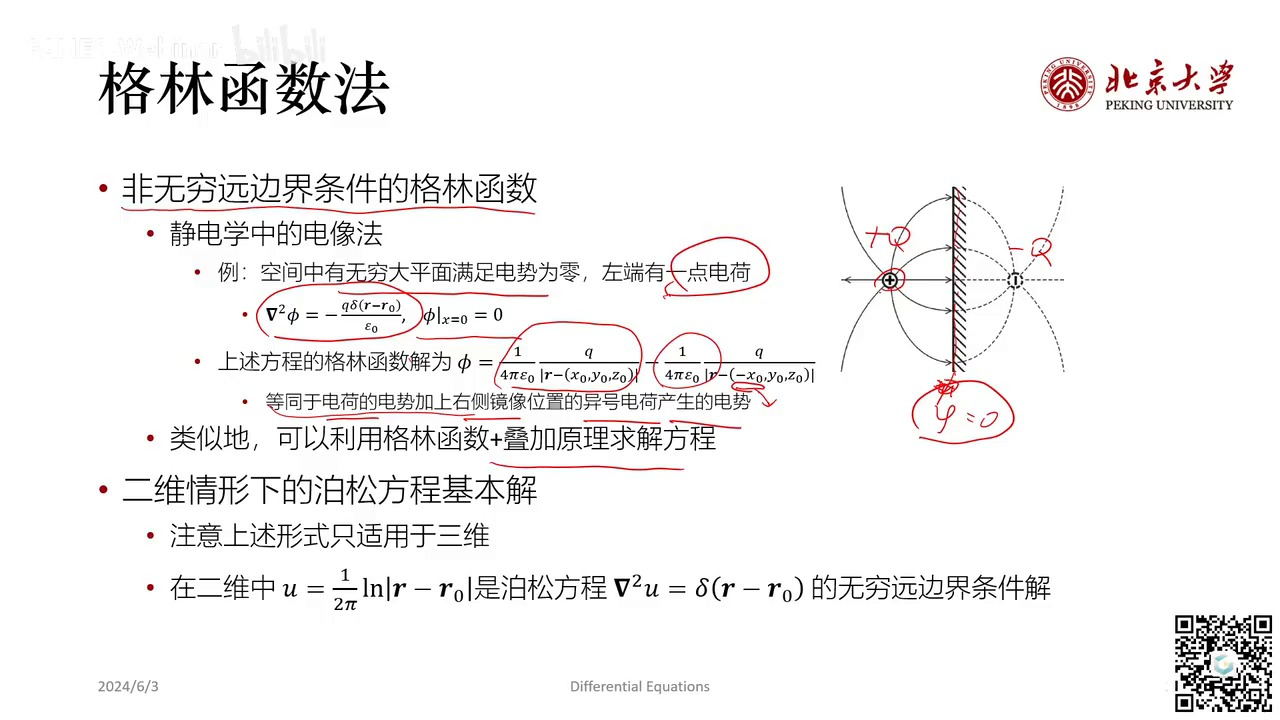
\includegraphics[width=0.92\textwidth]{figures/fig_23_green_image.jpg}
\caption{非无穷远边界条件下的格林函数：镜像法；二维泊松方程的基本解\vtag}
\end{figure}
\srcnote{00:57:00--00:57:15}
\end{minipage}


前面给出的都是无穷远边界条件下的格林函数解。非无穷远边界条件下呢？静电学中有镜像法。例：空间中有无穷大平面满足电势为零，左端有一点电荷，$\nabla^2\phi=-\frac{q\delta(\boldsymbol r-\boldsymbol r_0)}{\varepsilon_0}$，$\phi|_{x=0}=0$。上述方程的格林函数解为
\begin{equation}
\phi=\frac{1}{4\pi\varepsilon_0}\frac{q}{|\boldsymbol r-(x_0,y_0,z_0)|}-\frac{1}{4\pi\varepsilon_0}\frac{q}{|\boldsymbol r-(-x_0,y_0,z_0)|}.
\end{equation}
它相当于把 $\boldsymbol r_0$ 的 $x$ 坐标反号：等同于原电荷的电势，加上右侧镜像位置的异号电荷产生的电势，两者在平面上正好抵消。类似地，可以利用格林函数加叠加原理求解方程。

讲者提醒，无论无穷远还是非无穷远，上述形式都只适用于三维。在二维中，泊松方程 $\nabla^2u=\delta(\boldsymbol r-\boldsymbol r_0)$ 的无穷远边界条件解不是 $1/|\boldsymbol r-\boldsymbol r_0|$ 的形式，而是
\begin{equation}
u=\frac{1}{2\pi}\ln|\boldsymbol r-\boldsymbol r_0| .
\end{equation}

\subsection{格林恒等式}

\noindent\begin{minipage}{\textwidth}
\begin{figure}[H]
\centering
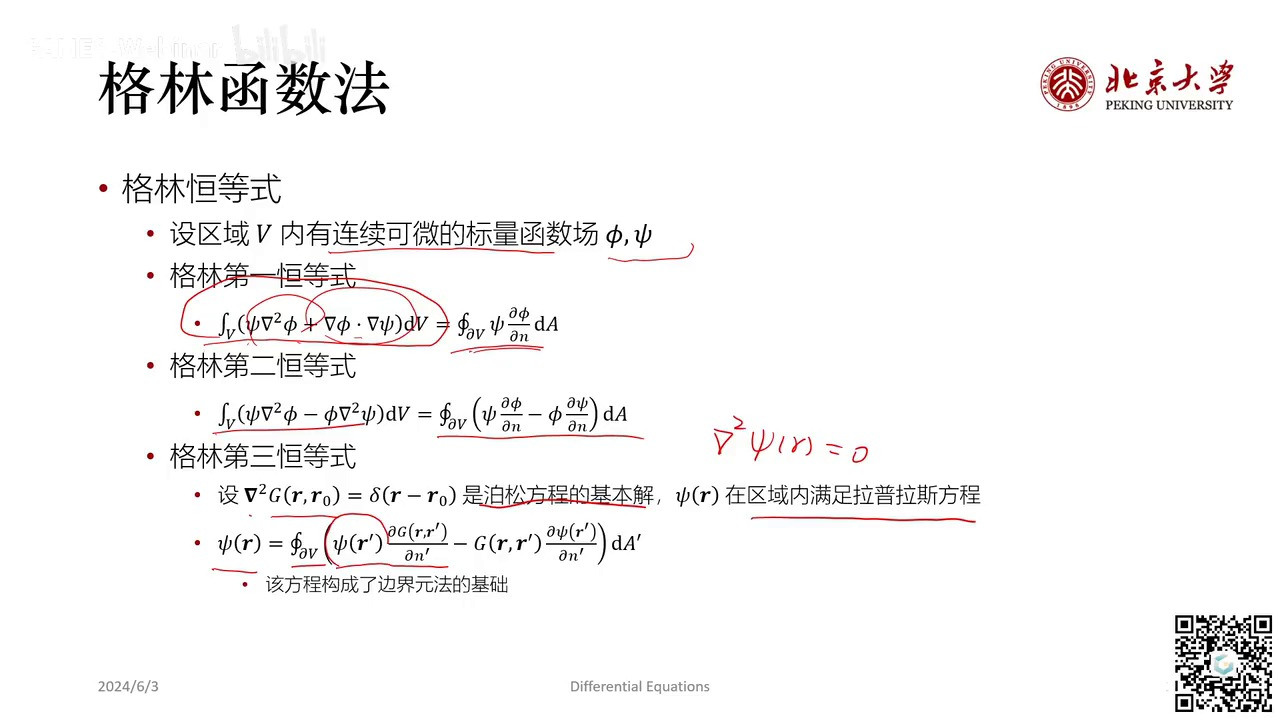
\includegraphics[width=0.92\textwidth]{figures/fig_24_green_identities.jpg}
\caption{格林第一、第二、第三恒等式\vtag}
\end{figure}
\srcnote{00:58:45--00:59:00}
\end{minipage}


设区域 $V$ 内有连续可微的标量函数场 $\phi,\psi$。格林第一恒等式：
\begin{equation}
\int_V(\psi\nabla^2\phi+\nabla\psi\cdot\nabla\phi)\,\mathrm{d}V=\oint_{\partial V}\psi\frac{\partial\phi}{\partial n}\,\mathrm{d}A .
\end{equation}
格林第二恒等式：
\begin{equation}
\int_V(\psi\nabla^2\phi-\phi\nabla^2\psi)\,\mathrm{d}V=\oint_{\partial V}\left(\psi\frac{\partial\phi}{\partial n}-\phi\frac{\partial\psi}{\partial n}\right)\mathrm{d}A .
\end{equation}
格林第三恒等式：设 $\nabla^2G(\boldsymbol r,\boldsymbol r_0)=\delta(\boldsymbol r-\boldsymbol r_0)$ 是泊松方程的基本解，$\psi(\boldsymbol r)$ 在区域内满足拉普拉斯方程，则
\begin{equation}
\psi(\boldsymbol r)=\oint_{\partial V}\left(\psi(\boldsymbol r')\frac{\partial G(\boldsymbol r,\boldsymbol r')}{\partial n'}-G(\boldsymbol r,\boldsymbol r')\frac{\partial\psi(\boldsymbol r')}{\partial n'}\right)\mathrm{d}A' .
\end{equation}
讲者解释：它相当于说，在空间中任取一个区域，如果知道区域边界上的值以及边界上的法向偏导数，就能得到区域内任意位置的 $\psi$。该方程构成了边界元法的基础。

\begin{warningbox}{“格林公式”不止一个}
上一讲（场论）中的格林公式是平面上环量与旋度的关系；这里的格林恒等式是关于拉普拉斯算子的体积分与面积分的关系，可以由高斯散度定理作用在 $\psi\nabla\phi$ 上推出。讲者在上一讲就提醒过二者不是一回事。
\end{warningbox}

\section{微分方程的数值解}

\subsection{常微分方程}

\noindent\begin{minipage}{\textwidth}
\begin{figure}[H]
\centering
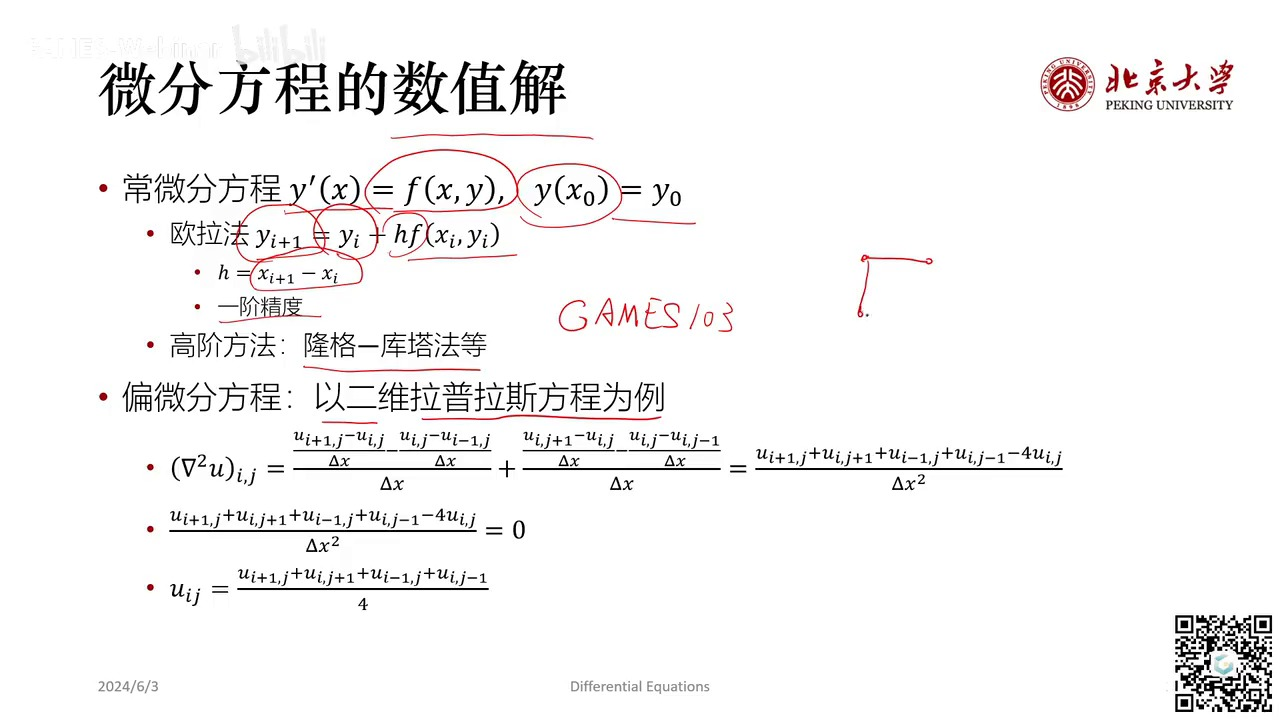
\includegraphics[width=0.92\textwidth]{figures/fig_25_numeric_ode.jpg}
\caption{常微分方程的欧拉法与二维拉普拉斯方程的有限差分\vtag}
\end{figure}
\srcnote{01:00:30--01:00:45}
\end{minipage}


对常微分方程 $y'(x)=f(x,y)$，$y(x_0)=y_0$，最简单的是欧拉法：
\begin{equation}
y_{i+1}=y_i+hf(x_i,y_i),\qquad h=x_{i+1}-x_i ,
\end{equation}
$h$ 为步长，这个方法只有一阶精度。通过一些手段提升精度，就得到高阶方法，例如龙格—库塔法等。

\begin{warningbox}{步长与稳定性}
讲义作者补充：欧拉法除了精度低，还可能不稳定。以 $y'=-ky$ 为例，欧拉法给出 $y_{i+1}=(1-hk)y_i$，当 $hk>2$ 时数值解会振荡发散，尽管真解单调衰减。物理模拟中刚度大的弹簧常让显式欧拉法“爆炸”，这就是原因，此时需要减小步长或改用隐式方法。
\end{warningbox}讲者说，偏微分方程的数值解法可以去看 GAMES103。

\subsection{偏微分方程：以二维拉普拉斯方程为例}

把区域划分为边长都是 $\Delta x$ 的正方形网格，用有限差分计算拉普拉斯算子。先用前向差分 $\frac{u_{i+1,j}-u_{i,j}}{\Delta x}$ 和后向差分 $\frac{u_{i,j}-u_{i-1,j}}{\Delta x}$ 近似一阶导数，再作差除以 $\Delta x$：
\begin{equation}
(\nabla^2u)_{i,j}\approx\frac{\frac{u_{i+1,j}-u_{i,j}}{\Delta x}-\frac{u_{i,j}-u_{i-1,j}}{\Delta x}}{\Delta x}+\frac{\frac{u_{i,j+1}-u_{i,j}}{\Delta x}-\frac{u_{i,j}-u_{i,j-1}}{\Delta x}}{\Delta x}=\frac{u_{i+1,j}+u_{i,j+1}+u_{i-1,j}+u_{i,j-1}-4u_{i,j}}{\Delta x^2}.
\end{equation}
令它等于零，化简得
\begin{equation}
u_{ij}=\frac{u_{i+1,j}+u_{i,j+1}+u_{i-1,j}+u_{i,j-1}}{4}.
\end{equation}
即中间格点的值等于周围四个格点值的平均。

\subsection{迭代求解}

\noindent\begin{minipage}{\textwidth}
\begin{figure}[H]
\centering
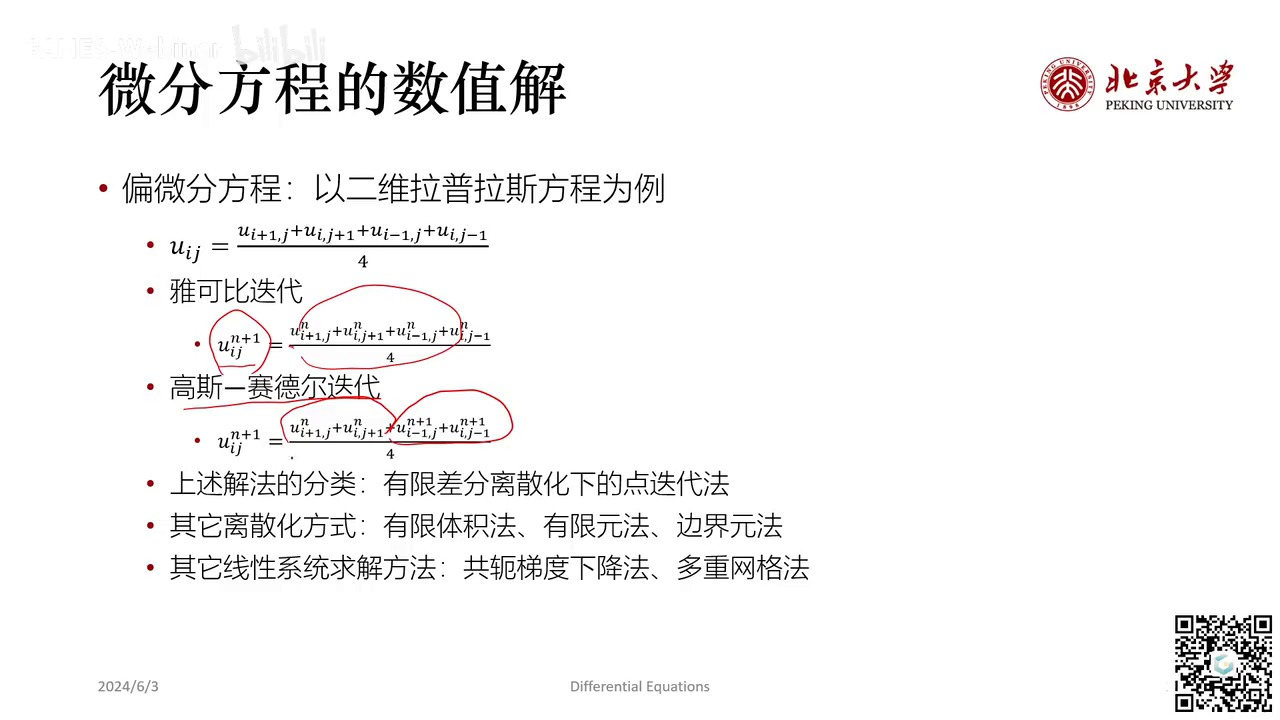
\includegraphics[width=0.92\textwidth]{figures/fig_26_numeric_iter.jpg}
\caption{雅可比迭代与高斯—赛德尔迭代\vtag}
\end{figure}
\srcnote{01:03:30--01:03:45}
\end{minipage}


雅可比迭代就用周围四个格点上一轮的值的平均来更新：
\begin{equation}
u_{ij}^{n+1}=\frac{u_{i+1,j}^n+u_{i,j+1}^n+u_{i-1,j}^n+u_{i,j-1}^n}{4}.
\end{equation}
讲者说这个方法的收敛效率稍慢。如何改进？非常简单，就得到高斯—赛德尔迭代：直接用 for 循环按顺序更新，一半的值用上一次的结果，另一半用这一次刚刚更新过的值：
\begin{equation}
u_{ij}^{n+1}=\frac{u_{i+1,j}^n+u_{i,j+1}^n+u_{i-1,j}^{n+1}+u_{i,j-1}^{n+1}}{4}.
\end{equation}
当两次迭代之间的变化足够小时，让算法停止就可以了。讲者说，这样就给出了求解二维拉普拉斯方程最简单的数值解法，这也是本讲的编程作业。

\noindent\begin{minipage}{\textwidth}
\begin{figure}[H]
\centering
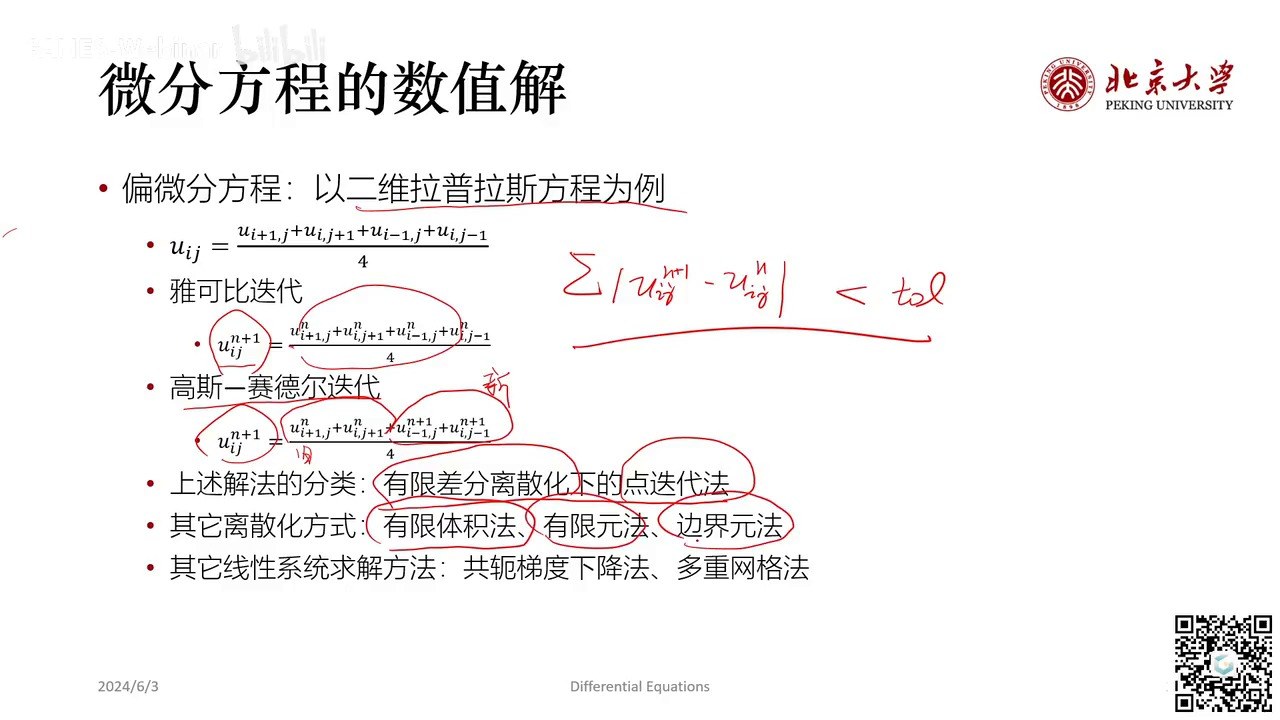
\includegraphics[width=0.92\textwidth]{figures/fig_27_numeric_note.jpg}
\caption{讲者在迭代公式旁的批注\vtag}
\end{figure}
\srcnote{01:04:30--01:04:45}
\end{minipage}


上述解法的分类是：有限差分离散化下的点迭代法。其它离散化方式有有限体积法、有限元法、边界元法；其它线性系统求解方法有共轭梯度下降法、多重网格法等。

\begin{practicebox}{动手实现}
讲义作者建议按讲者布置的编程作业做一个小实验：在 $64\times 64$ 的网格上，把边界一侧设为 $1$、其余边界设为 $0$，内部初始化为 $0$，分别用雅可比迭代和高斯—赛德尔迭代求解，记录残差降到 $10^{-6}$ 以下所需的迭代次数。可以观察到高斯—赛德尔大约只需雅可比的一半次数，但两者都随网格变细而迅速变慢，这正是多重网格法要解决的问题。
\end{practicebox}

\section{小结}

讲者解释了这节课为什么“承上启下”：我们巧妙地把二维拉普拉斯方程通过空间离散化，转换成了离散格点值之间的一组恒等关系，也就是一个巨大的矩阵方程。通过离散化，偏微分方程变成了线性方程组；下一讲就要讲如何求解这样的线性系统。

\begin{knowledgebox}{全讲回顾}
常微分方程的几种解法，核心是“猜形式”与“换变量”：分离变量、常数变易、变量代换、指数试探解。偏微分方程按二阶项的判别式分为双曲、抛物、椭圆三类，分别对应波动、热传导和拉普拉斯方程。分离变量法给出傅里叶展开形式的解，在球坐标下就得到球谐函数；格林函数法先求点源响应再叠加；数值法把连续问题离散成代数问题。
\end{knowledgebox}

\end{document}
